% !TEX program = xelatex
% 2026 극지 빅데이터-인공지능 활용 경진대회 예선 분석 보고서
% 컴파일: xelatex main.tex (2회) 또는 latexmk -xelatex main.tex
\documentclass[10pt]{article}

% ---------- 레이아웃 ----------
\usepackage[a4paper,top=20mm,bottom=20mm,left=18mm,right=18mm]{geometry}
\usepackage{amsmath}
\usepackage{amssymb}
\usepackage{fontspec}
\usepackage{xeCJK}
% 한국어는 단어 사이 공백으로 띄어쓰기하므로 CJKspace를 켜서 공백을 보존한다(기본값 false는 중국어·일본어용).
\xeCJKsetup{CJKspace=true}
\usepackage{graphicx}
\usepackage{booktabs}
\usepackage{array}
\usepackage{float}
\usepackage{xcolor}
\usepackage{caption}
\usepackage{subcaption}
\usepackage{titlesec}
\usepackage{enumitem}
\usepackage{multicol}
\usepackage[hidelinks]{hyperref}

% ---------- 색 ----------
\definecolor{accent}{HTML}{1F3A5F}
\definecolor{rule}{HTML}{2C3E50}
\definecolor{softgray}{HTML}{5B6670}

% ---------- 폰트 (본문=Noto Serif CJK KR, 제목=Pretendard) ----------
\setmainfont{Noto Serif CJK KR}[
  UprightFont={Noto Serif CJK KR}, BoldFont={Noto Serif CJK KR Bold},
  AutoFakeSlant=0.18]
\setCJKmainfont{Noto Serif CJK KR}[
  UprightFont={Noto Serif CJK KR}, BoldFont={Noto Serif CJK KR Bold},
  AutoFakeSlant=0.18]
\newfontfamily\headfont{Pretendard}[
  Path=/home/willy010313/.fonts/,
  UprightFont=Pretendard-SemiBold.otf,
  BoldFont=Pretendard-Black.otf]
\newCJKfontfamily\cjkhead{Pretendard}[
  Path=/home/willy010313/.fonts/,
  UprightFont=Pretendard-SemiBold.otf,
  BoldFont=Pretendard-Black.otf]

% 한글 줄바꿈: 한국어는 공백 기반 띄어쓰기이므로 글자단위 줄바꿈(XeTeXlinebreaklocale) 미사용.
% xeCJK 기본 공백 처리로 단어 사이 간격을 보존한다.
\setlength{\parindent}{1.05em}
\setlength{\parskip}{0.15em}
\linespread{1.06}

% ---------- 섹션 서식 ----------
\titleformat{\section}
  {\headfont\cjkhead\large\bfseries\color{accent}}{\thesection}{0.6em}{}
\titleformat{\subsection}
  {\headfont\cjkhead\normalsize\bfseries\color{rule}}{\thesubsection}{0.55em}{}
\titlespacing*{\section}{0pt}{1.4ex}{0.7ex}
\titlespacing*{\subsection}{0pt}{1.0ex}{0.45ex}

% ---------- 캡션 ----------
\captionsetup{font=small,labelfont={bf,color=accent},labelsep=period,
  justification=justified,singlelinecheck=false}
\captionsetup[sub]{font=footnotesize}

% ---------- 표 ----------
\renewcommand{\arraystretch}{1.18}
\newcommand{\tabhead}[1]{\textbf{#1}}

% ---------- 제목부 커스텀 ----------
\begin{document}
\pagestyle{plain}

% ===== 제목 블록 =====
\begin{center}
{\headfont\cjkhead\LARGE\bfseries\color{accent}%
관측기반 GeoAI를 이용한 영구동토 활동층 두께 예측:\\[2pt]
2D 지도 · 얕은 3D 열구조 · 전이 일반화 · 보정 불확실성\par}
\vspace{6pt}
{\headfont\cjkhead\normalsize\color{softgray}%
2026 극지 빅데이터-인공지능 활용 경진대회 예선 분석 보고서\par}
\vspace{2pt}
{\color{softgray}\rule{0.42\textwidth}{0.6pt}}
\end{center}
\vspace{2pt}

% ===== 초록 =====
\begin{quote}
\small
\noindent\textbf{초록.}\;
영구동토 활동층 두께(active layer thickness, ALT)는 지반 안정성과 탄소 순환을 좌우하는 1차 상태변수이나, 현장 관측이 소수 사이트에 초집중돼 광역 추정과 지역 간 전이가 어렵다.
본 연구는 희소한 지점 관측과 광역 지형·기후 공변량을 결합하는 관측기반 GeoAI 프레임워크를 제안한다.
물리 앵커(Stefan $a{+}E\sqrt{\mathrm{TDD}}$), 기계학습 토너먼트, 물리 pseudo-label 증강, 정통 지구통계 보간(크리깅)을 누설통제 프로토콜(공간블록 GroupKFold, leave-one-region-out) 아래에서 동일하게 채점하고, 분위 회귀와 conformal 보정으로 통계적으로 유효한 예측구간을 부여한다.
알래스카 in-domain 검증에서 신경망·부스팅·물리식이 모두 $14\text{--}16\,\mathrm{cm}$ 대역에 수렴하고, 위경도 2피처 대조군이 정교한 물리·SAR 공변량 조합을 능가한다. 이는 병목이 모델 용량이 아니라 공변량 정보량임을 직접 보인다.
지역 간 전이에서는 순수 기계학습과 공간보간이 붕괴($34\text{--}51\,\mathrm{cm}$)하는 반면 물리 앵커만 하한($21\,\mathrm{cm}$)을 유지하며, 증강·다중충실도 구조의 순가치는 물리 정확도에 조건부임을 정량화한다.
conformal 보정은 $90\%$ 커버리지를 $44.6\%$에서 $93.4\%$로 교정한다.
KPDC 콘슬 지중온도로 공변량 backbone과 물성 이질성을 현장 검증한다.
기여는 전이 붕괴의 정량 진단, 배포 가능한 물리 앵커 해법, 보정 불확실성, 정보병목 기반 데이터 수집 우선순위 제시이다.
\par
\vspace{2pt}
\noindent\textbf{핵심어.}\; 영구동토, 활동층 두께, GeoAI, 물리 앵커, 전이 일반화, 보정 불확실성, 지구통계.
\end{quote}

\begin{multicols}{2}

% =====================================================================
\section{서론}
% =====================================================================

\subsection{배경과 문제}
영구동토 상부에는 여름에 융해하고 겨울에 재동결하는 층이 있다. 이 계절 융해층의 최대 깊이가 활동층 두께(ALT)이다. ALT는 지반 안정성, 탄소 순환, 수문 순환을 좌우하는 1차 상태변수이다. 활동층이 깊어지면 동결 상태로 격리돼 있던 유기탄소가 분해 가능한 상태로 노출되고 지반 침하와 열카르스트가 진행된다. 따라서 ALT의 공간 분포와 시간 변화를 정량화하는 것은 극지 환경 감시의 핵심 과제이다.

ALT는 넓은 면적에서 직접 관측하기 어렵다. 현장 조사는 탐침 또는 시추로 측정하며 공간적으로 희소하다. 이 때문에 희소한 지점 관측과 광역 공변량을 결합해 미관측 지역으로 확장하는 통계·기계학습 접근이 표준이 됐다. 그러나 관측이 소수 사이트에 초집중된 특성 때문에 두 가지 난제가 남는다. 첫째, 무엇이 예측을 실제로 지배하는지(정보병목)가 불분명하다. 둘째, 한 지역에서 학습한 모델이 다른 영구동토 지대로 일반화되는지(전이)가 검증되지 않았다.

\subsection{기존 연구의 한계}
기존 영구동토 모델링은 세 계열로 나뉜다. 물리 순방향 시뮬레이션(GIPL2/SNAP 계열)은 열전도 방정식을 적분해 지온을 산출하나, 관측 라벨로의 직접 검증과 지역 간 전이 성능이 체계적으로 평가되지 않았다. 관측기반 통계 제품(ESA CCI, Obu 등 2019)은 광역 지도를 제공하나 예측구간(불확실성)이 탑재되지 않아 어디까지 믿을 수 있는지를 사용자가 판단하기 어렵다. 최근의 물리정보 신경망(InterPIGNN, PI-LSTM 등)은 방법론 신규성에 초점을 두나 누설을 통제한 전이 벤치마크와 보정된 커버리지 보고가 드물다. 요약하면 기존 연구는 순방향 시뮬레이션 위주이며, 전이학습이 정량 평가되지 않았고, 배포에 필요한 보정 불확실성이 결여돼 있다.

\subsection{본 연구의 기여}
본 연구는 관측을 1차 근거로 삼는 GeoAI 프레임워크로 다음을 기여한다.

\begin{enumerate}[leftmargin=1.25em,itemsep=1pt,topsep=2pt]
\item \textbf{전이 붕괴의 정량 진단.} 순수 기계학습·공간보간이 지역 간에 붕괴하고 물리 앵커만 하한을 지킨다는 것을, 구조 정교화의 부정 결과를 포함해 통제된 게이트에서 정량화한다.
\item \textbf{배포 가능한 하이브리드 해법.} 온도-깊이 관계가 지역 간 유지되는 Stefan 앵커를 전이 하한으로 두고, 적용가능 영역(AOA) 표기를 결합한다.
\item \textbf{보정 불확실성.} conformal 보정으로 통계적으로 유효한 예측구간을 부여하고 그 범위와 한계를 명시한다.
\item \textbf{정보병목 진단과 데이터 우선순위.} 위경도 대조군 실험으로 병목이 공변량 정보량임을 밝히고, 면적검증·target 라벨·조밀 지중온도라는 실효 지렛대를 제시한다.
\end{enumerate}

정확도 경쟁 하나만을 목표로 삼지 않는다. 정보병목, 신뢰가능성, 전이 한계를 함께 규명하는 것이 본 연구의 정체성이다.

% =====================================================================
\section{데이터}
% =====================================================================
학습·검증 자료는 관측 라벨, 공변량, 물리관측, 현장검증(KPDC)의 네 축이다. 통합 스키마는 고유 위치 17{,}423셀(공변량 코어 34종)로 구성했다. 이 중 라벨과 공변량이 모두 유효한 알래스카 셀 13{,}606개가 in-domain 학습·평가의 기준 표본이다. 관측 ALT는 통합 셀 기준 평균 약 $50\,\mathrm{cm}$, 표준편차 약 $20\,\mathrm{cm}$이며 대부분 알래스카에 편중된다(알래스카 부분집합만 보면 표준편차 약 $17\,\mathrm{cm}$). 관측이 소수 사이트(83개 $0.5^\circ$셀)에 초집중된 특성은 본 연구의 설계와 해석 전반을 규정한다.

\begin{table}[H]
\centering
\footnotesize
\caption{관측 라벨과 주요 자료원. 규모는 집계 후 셀 수이다.}
\label{tab:data}
\begin{tabular}{@{}p{1.85cm}p{2.3cm}r@{}}
\toprule
\tabhead{자료원} & \tabhead{대상·지역} & \tabhead{규모} \\
\midrule
CALM / ABoVE & 알래스카 활동층 & 13{,}606 \\
ALLena & 레나델타 thaw depth & 3{,}037 \\
ABoVE 캐나다 & 캐나다 활동층 & 726 \\
GTN-P & 다지역 지중온도(보조) & 수십 \\
KPDC 콘슬 & 수어드반도 지온·코어 & 37+18 \\
\bottomrule
\end{tabular}
\end{table}

\textbf{공변량 14종(전이-강건 코어).} 전이 실험의 공정 비교를 위해 전 지역에서 결측 없이 확보되는 지형·기후 14종을 코어 입력으로 고정했다. 지형(DEM 파생) 6종은 표고·경사·사면 방위(sin·cos)·지형위치지수(TPI)·거칠기이고, 기후(ERA5-Land 파생) 8종은 연평균기온·융해도일(TDD)·동결도일(FDD)·$\sqrt{\mathrm{TDD}}$·최난월·최한월 기온·1층 토양온도·적설수당량이다. 토양(SoilGrids), InSAR, PolSAR, ESA CCI는 스키마에 포함하나 지역별 결측(InSAR·PolSAR는 알래스카 외 0\%) 때문에 전이 입력에서는 제외한다.

\textbf{물리관측.} InSAR 침하 유도 ALT와 PolSAR 유도 ALT는 알래스카 국한으로 면적평균 검증의 후보이다. ESA CCI ALT 제품(25년 다년평균)은 관측과 상관 $r\approx0.53$이며 독립 벤치마크로만 사용한다.

\textbf{KPDC 현장자료(주 활용).} 대회 요건에 따라 KPDC 자료를 주된 검증·해석 축으로 사용한다. 수어드반도 Council 사이트의 콘슬 8--16층 일별 지중온도 프로파일 19종, 코어 thaw depth 18개(코어길이 72--88\,cm), AWS 기상관측을 편입했다. KPDC 콘슬은 알래스카 in-domain 점검증(최근접 학습 셀 0.97\,km)으로 사용하며 전이 근거로는 쓰지 않는다.

\end{multicols}

\begin{figure*}[t]
\centering
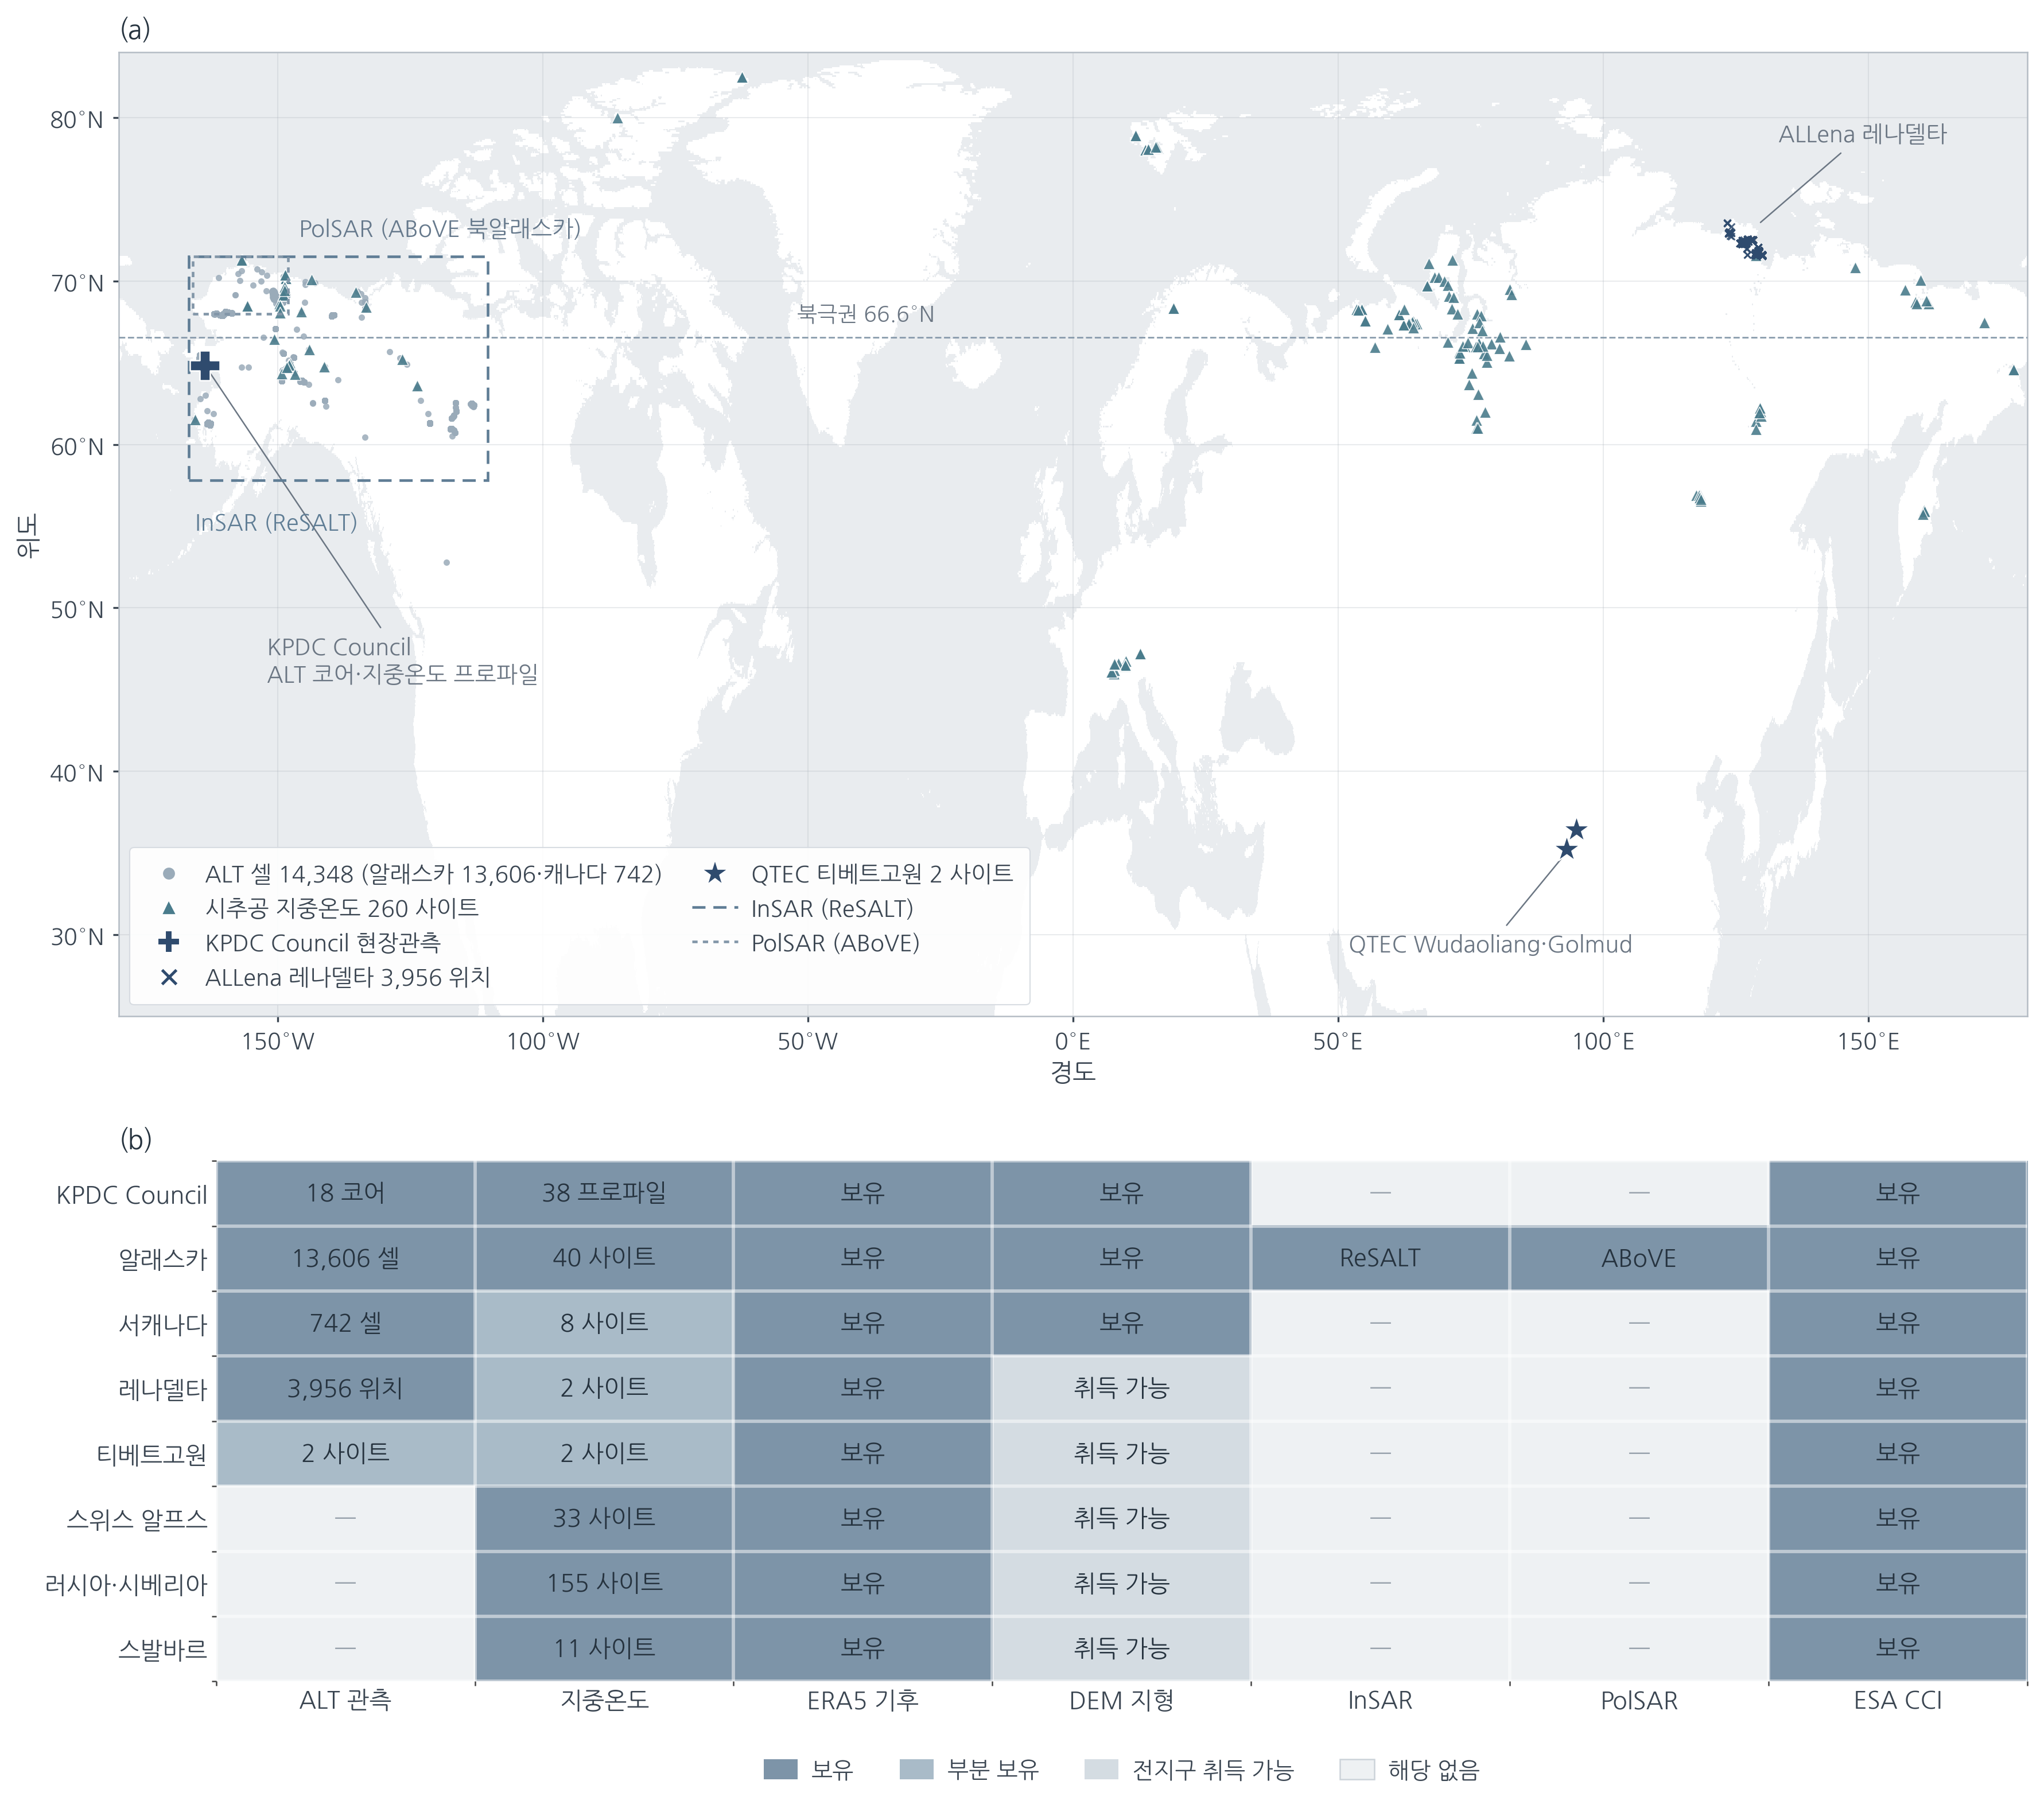
\includegraphics[width=0.9\textwidth]{../../outputs/maps/data_inventory_world.png}
\caption{데이터 인벤토리. 관측 라벨·공변량·물리관측·KPDC 현장자료의 지리 분포. 관측 라벨은 알래스카·레나델타·캐나다의 소수 사이트에 초집중되며, 이 표본 편중이 전이 난제의 구조적 원인이다.}
\label{fig:inventory}
\end{figure*}

\begin{multicols}{2}

% =====================================================================
\section{방법}
% =====================================================================
각 기법의 원리를 간결히 정의한다.

\textbf{물리 앵커(Stefan).} Stefan 방정식은 활동층 융해를 열전도 문제로 근사해 $\mathrm{ALT}=a+E\sqrt{\mathrm{TDD}}$ 형태를 준다. $\mathrm{TDD}$는 누적 융해도일, $E$는 열·수분 물성을 묶은 계수, $a$는 절편이다. 온도-깊이 관계가 지역 간 이동 시에도 유지되므로 전이의 하한을 담당한다. 계수 $E$는 각 fold의 학습 표본에서만 추정해(fold-safe) 누설을 막는다.

\textbf{기계학습 토너먼트.} 지형·기후 공변량으로 ALT를 직접 회귀하는 모델군을 비교한다. 트리 부스팅(HistGBM·LightGBM·XGBoost·CatBoost)과 신경망(MLP·FT-Transformer·TabM)을 동일 fold·동일 입력으로 채점한다. 신경망 입력은 fold-safe z-score로 표준화한다.

\textbf{물리 pseudo-label 증강.} 타깃 지역(레나·캐나다)에 Stefan 유도값을 pseudo-label로 붙여 학습을 보강하고 증강 비율 $r$을 스윕한다. 대조군으로 알래스카 평균 상수를 라벨로 붙이는 placebo를 둬서 개선이 물리 정보에서 오는지 단순 앵커링에서 오는지 분리한다.

\textbf{source-aware 다중충실도.} 자료원별 관측모델 $y_s = A_s[z] + b_s + \varepsilon_s$로 공유 잠재장 $z$, 소스 편향 $b_s$, 소스 분산 $\sigma_s$를 함께 추정한다. 병합과 달리 자료원 신뢰도를 명시적으로 모델링한다.

\textbf{공간보간(크리깅).} 정통 지구통계 baseline이다. 보통 크리깅(OK)은 변동도로 공간자기상관을 모델링해 미관측점을 내삽하고, 회귀 크리깅(RK)은 공변량 회귀 잔차를 크리깅한다. IDW는 거리역가중이다. 물리·기계학습과 동일 프로토콜로 비교한다.

\textbf{누설통제.} 공간자기상관 때문에 무작위 분할은 성능을 크게 낙관한다. 이를 막기 위해 (a) $0.5^\circ$ 공간블록 GroupKFold(in-domain), (b) leave-one-region-out(LORO, 매크로 지역 비가중평균 게이트), (c) leave-source-out을 사용한다. 라벨 파생 7종(셀내 표준편차·최소·최대 등)은 영구 제외하고 fold-safe Stefan $E$를 강제한다. LORO 게이트를 매크로 지역 비가중평균으로 둔 이유는 표본이 알래스카에 편중돼 셀 가중평균이 사실상 in-domain 점수로 수렴하기 때문이다. 지역 단위 평균은 전이 성능을 표본 편중과 분리해 측정한다. 이 무결성은 누설방지 단위테스트 16개로 상시 검증한다.

\textbf{보정 불확실성.} 분위 회귀로 예측구간을 얻은 뒤 conformalized quantile regression(CQR)으로 학습 블록 내부 보정을 적용해 목표 커버리지를 맞춘다. 원 분위구간의 과신을 후보정한다.

\textbf{적용가능 영역(AOA).} 비유사도지수(DI)로 예측점이 학습 공변량 공간에서 얼마나 떨어져 있는지를 정량화하고 DI가 높은 외삽 영역을 표기한다.

% =====================================================================
\section{결과}
% =====================================================================

\subsection{정확도와 정보병목}
알래스카 공간블록 검증에서 최상위 모델군은 좁은 대역에 몰린다(표~\ref{tab:indomain}). 신경망·부스팅·물리식이 모두 약 $14\text{--}16\,\mathrm{cm}$ 대역에 들어오며, 모델 교체로 얻는 이득이 seed 잡음 범위 안이다. 따라서 정확도의 병목은 모델 용량이 아니다.

\begin{table}[H]
\centering
\footnotesize
\caption{in-domain ALT 예측(알래스카 공간블록, 3-seed).}
\label{tab:indomain}
\begin{tabular}{@{}lrl@{}}
\toprule
\tabhead{방법} & \tabhead{RMSE(cm)} & \tabhead{비고} \\
\midrule
MLP(앙상블 OOF) & 14.37 & 신경망 최상 \\
TabM(앙상블 OOF) & 14.40 & MLP와 동률 \\
Stefan 물리($\sqrt{\mathrm{TDD}}$) & 14.56 & 물리식 단독 \\
CatBoost & 15.61 & GBM 대표 \\
HistGBM & $\approx$17.1 & GBM 하위 \\
\bottomrule
\end{tabular}
\end{table}

병목의 성격은 위경도 대조군 실험이 직접 드러낸다(표~\ref{tab:ablation}). 셀 단위 feature-group ablation에서 위경도 2피처만 쓴 대조군(Mloc)이 물리 공변량 조합보다 앞선다. 위도가 기후 이상을 대리하는 것만으로 정교한 물리·SAR 공변량 조합을 넘는다. 이는 현재 공변량이 담는 정보량 자체가 상한이라는 직접 증거이다. 지형 단독은 오히려 악화되는데, 이는 지형이 무관해서가 아니라 $9\,\mathrm{km}$ 기후 셀에 $30\,\mathrm{m}$ DEM 정보가 이미 평균돼 미세지형 신호가 희석되기 때문이다.

\begin{table}[H]
\centering
\footnotesize
\caption{feature-group ablation(14{,}348셀). skill은 상수 대비 개선.}
\label{tab:ablation}
\begin{tabular}{@{}lrr@{}}
\toprule
\tabhead{구성} & \tabhead{LORO RMSE(cm)} & \tabhead{skill} \\
\midrule
Mloc 위경도(대조) & 15.72 & 0.147 \\
M4 +InSAR & 16.09 & 0.127 \\
M1 기후 & 16.45 & 0.108 \\
M3 기후+지형 & 16.94 & 0.082 \\
M2 지형 단독 & 19.40 & $-0.052$ \\
\bottomrule
\end{tabular}
\end{table}

\subsection{전이: 물리 앵커만 지탱한다}
알래스카 학습 후 레나·캐나다로 넘어가는 LORO 게이트에서 순수 기계학습은 붕괴하고 Stefan 앵커만 하한을 유지한다(표~\ref{tab:transfer}). 트리 부스팅은 알래스카에 과적합돼 전이에서 $34\text{--}38\,\mathrm{cm}$로 파탄한다. Stefan 앵커는 온도-깊이 물리 관계가 지역 간 유지되므로 $21\text{--}22\,\mathrm{cm}$ 대역을 지킨다.

정통 지구통계도 전이에서 붕괴한다. in-domain에서는 OK($15.77$)·IDW($15.80$)가 공변량 GBM($17.73$)과 경쟁하나, 전이에서는 OK $29.40$, RK $36.30$, IDW $50.92$로 무너진다. 원인은 변동도가 지역마다 다르다는 데 있다(range·sill의 지역 편차). 이는 covariate shift의 공간통계판이다. OK의 레나 전이가 겉으로 낮은 것은 실력이 아니라 변동도 range 밖에서 학습 전역평균으로 회귀하는 아티팩트이다.

\begin{table}[H]
\centering
\footnotesize
\caption{in-domain 대 LORO 게이트 전이(RMSE, cm).}
\label{tab:transfer}
\begin{tabular}{@{}lrr@{}}
\toprule
\tabhead{방법} & \tabhead{in-domain} & \tabhead{LORO 게이트} \\
\midrule
Stefan(물리 앵커) & 14.46 & \textbf{21.26} \\
OK(보통 크리깅) & 15.77 & 29.40 \\
RK(회귀 크리깅) & 17.23 & 36.30 \\
GBM(공변량) & 17.74 & 41.37 \\
MLP(직접) & 14.37 & 34.24 \\
CatBoost(직접) & 15.61 & 38.42 \\
IDW & 15.80 & 50.92 \\
\bottomrule
\end{tabular}
\end{table}

구조 정교화는 전이를 개선하지 못한다(부정 결과를 담백히 보고한다). source-aware 다중충실도(S6)는 LORO $21.53\text{--}21.84\,\mathrm{cm}$로 baseline(naive pooling $21.11$·앵커 $21.26$)을 못 넘는다. 다만 $b_{\text{stefan}}\approx0$이 실제 bias와 정합하고 $b_{\text{cci}}$가 과소추정을 드러내 자료원 식별성 한계를 정량화하는 진단 가치가 있다. mixture-of-physics(S8)는 LORO $29.22\,\mathrm{cm}$로 단일 Stefan을 못 이기는데, 정확한 전문가가 Stefan뿐이라(물리 5종 상관 $0.89\text{--}1.00$) 게이트 전환이 오히려 편향 전문가로 이동하기 때문이다. 이는 전이에서 전문가 선택 불가능성의 정량 증거이다.

\subsection{증강: 언제 돕고 언제 해치는가}
증강·구조 6계열을 동일 게이트로 종합 비교했다(표~\ref{tab:aug}). 핵심 함의는 세 가지이다. 첫째, 어떤 증강·구조도 LORO 전이에서 Stefan 앵커($21.26$)를 유의하게 넘지 못한다. pool\_mlp $21.11$은 동률이나 in-domain을 파괴하고($16.18$) target 셀 보조관측을 거리버퍼 없이 학습에 넣는 transductive 설계라 inductive 게이트로 비교할 수 없다. 둘째, 증강 이득 대부분은 물리 정보가 아니라 target 앵커링에서 온다. placebo 대조로 순가치를 분리하면 증강은 물리가 정확하고 bias 큰 전이·약한 base 모델일수록 순가치가 크다(Canada는 placebo가 악화인데 Stefan은 개선). 셋째, 부정확 물리(Kudryavtsev)를 pseudo-label로 넣으면 $r$을 키울수록 악화된다. 증강 자체가 아니라 물리 정확도가 부호를 결정한다.

in-domain 최저는 잔차학습(Stefan 앵커$+\lambda\cdot$저용량 잔차)의 $13.33\,\mathrm{cm}$이나, 이 구조도 전이에서는 $\lambda>0$ 전 구간이 게이트를 악화시켜($21.26{\to}21.83$) 부정 결과이다.

\begin{table}[H]
\centering
\footnotesize
\caption{증강·구조 종합 비교(S11 발췌). *는 transductive.}
\label{tab:aug}
\begin{tabular}{@{}lrrl@{}}
\toprule
\tabhead{방법} & \tabhead{in-dom} & \tabhead{LORO} & \tabhead{판정} \\
\midrule
Stefan 앵커 & 14.46 & \textbf{21.26} & 채택 \\
MLP 앙상블 & 14.37 & 34.24 & in-dom 기준 \\
잔차학습 & \textbf{13.33} & 21.83 & 전이 부정 \\
source-aware & 14.35 & 21.84 & 부정 \\
mixture & 14.97 & 29.22 & 진단만 \\
pool(병합)* & 16.18 & 21.11 & 미채택 \\
\bottomrule
\end{tabular}
\end{table}

\subsection{신뢰가능성: 보정 불확실성}
분위 CatBoost의 원 예측구간은 심하게 과신한다(cov90 $44.6\%$). 학습 블록 내부 CQR 보정 후 목표 커버리지에 도달한다(표~\ref{tab:uq}). 셀 단위 재분석에서도 raw $56.1\%\to$CQR $85.9\%$로 같은 방향의 과신 교정이 확인된다. 다만 이 보정은 in-domain 보장이며 전이 커버리지 보장은 아니다(전이에서는 전 방법이 과신). AOA DI-구간에서 비유사도가 커질수록 오차가 증가하고(저DI 약 $13\to$고DI 약 $30\,\mathrm{cm}$) 커버리지가 낮아져 외삽 영역을 표기한다.

점검증 자체에 대표성 하한이 있다. 단일 탐침 정밀도(약 $\pm3\,\mathrm{cm}$)와 셀 내 자연 공간변동(툰드라 표준편차 $9\text{--}12\,\mathrm{cm}$)을 결합하면 약 $10\text{--}12\,\mathrm{cm}$의 비가역 하한이 나온다. 완벽한 모델도 단일점 평가에서 이 잡음을 없앨 수 없다. 현재 $15.7\text{--}16.9\,\mathrm{cm}$는 이 하한에 근접한다.

\begin{table}[H]
\centering
\footnotesize
\caption{conformal 보정 전후 90\% 커버리지.}
\label{tab:uq}
\begin{tabular}{@{}lrr@{}}
\toprule
\tabhead{설정} & \tabhead{커버리지} & \tabhead{평균 폭(cm)} \\
\midrule
raw quantile & 44.6\% & 14.7 \\
CQR conformal & \textbf{93.4\%} & 53.6 \\
\bottomrule
\end{tabular}
\end{table}

\subsection{얕은 3D · 시계열 · 계절내 $D(t)$}
알래스카 $0\text{--}3\,\mathrm{m}$ 실측으로 학습한 GBM 조건장이 온도장을 재현한다(RMSE $2.66^\circ\mathrm{C}$, $R^2\,0.47$). 온도장 검증은 성립하나 $0^\circ\mathrm{C}$ 등온면을 ALT로 환산한 값은 관측과 $r\approx0.28$로 절대정합은 미완이며, 온도장 재현과 ALT 환산이 별개의 검증 단계임을 명시한다.

연별 timelapse는 재학습 없이 2010--2024 연별 ALT 지도 15장을 연도별 forcing$\times$연도별 라벨로 시간 정합해 렌더했다. 연도 홀드아웃 RMSE는 $14.97\,\mathrm{cm}$($R^2\,0.34$)이나, within-site 연 anomaly는 예측 불가하다(corr $+0.059$, anomaly skill $-0.003$). 연도 간 지도 차이는 그해 forcing의 반영일 뿐 위치별 연 변동 예측력이 아니다.

계절내 융해진행 $D(t)$는 연도간 최대 ALT 외삽(예측불가)이 아니라 계절곡선 예측으로 재정의했다. KPDC 콘슬 일별 지중온도에서 표층 연결 $0^\circ\mathrm{C}$ 등온선의 계절곡선을 유도했다. 계절내 $D(t)$는 예측 가능한 계절 구조를 갖는다(Stefan deepening 구간 $R^2\,0.31\text{--}0.57$). 이는 연도간 anomaly의 corr $0.06$과 대조된다. 다만 common-support·물리위치 fold 통제 후 7일 persistence($17.5\,\mathrm{cm}$)가 강baseline이라 Stefan($40.8$)·GRU($46.6$)는 이를 못 넘는다(2년 소표본·지온 유래 forcing 한계). 최대깊이 도달일은 단조 물리식으로는 원리적으로 불가하고 GRU만 내부 peak를 예측할 수 있다. 결론은 시간 성능이 방법이 아니라 문제정의·데이터밀도에 의존한다는 것이다.

\subsection{KPDC 현장 검증}
콘슬 지중온도 프로파일에서 표층 연결 $0^\circ\mathrm{C}$ 등온선으로 ALT를 유도하고 코어·물리·학습모델과 대조했다. 심부 16층 프로파일 배치가 필요해 38시즌 중 23건이 우측검열이라 구간검열 정량표를 함께 제시한다. ERA5-Land $\sqrt{\mathrm{TDD}}$가 콘슬 현장과 정합하며(bias $\sim0.1$) 공변량 backbone의 현장 검증이 성립한다. 단일 $E$ Stefan은 콘슬을 약 $1.7$배 과대예측하는데, 이는 지역 물성에 따른 $E(x)$ 필요성의 동기이다. 같은 사이트에서도 관측 방식(탐침·코어·심부 유도)에 따라 $35\text{--}153\,\mathrm{cm}$로 벌어져 점검증의 대표성 잡음이 지배함을 확인한다.

\end{multicols}

% ===== 그림 묶음 1: 정확도·정보병목·전이 =====
\begin{figure*}[t]
\centering
\begin{subfigure}[t]{0.485\textwidth}
  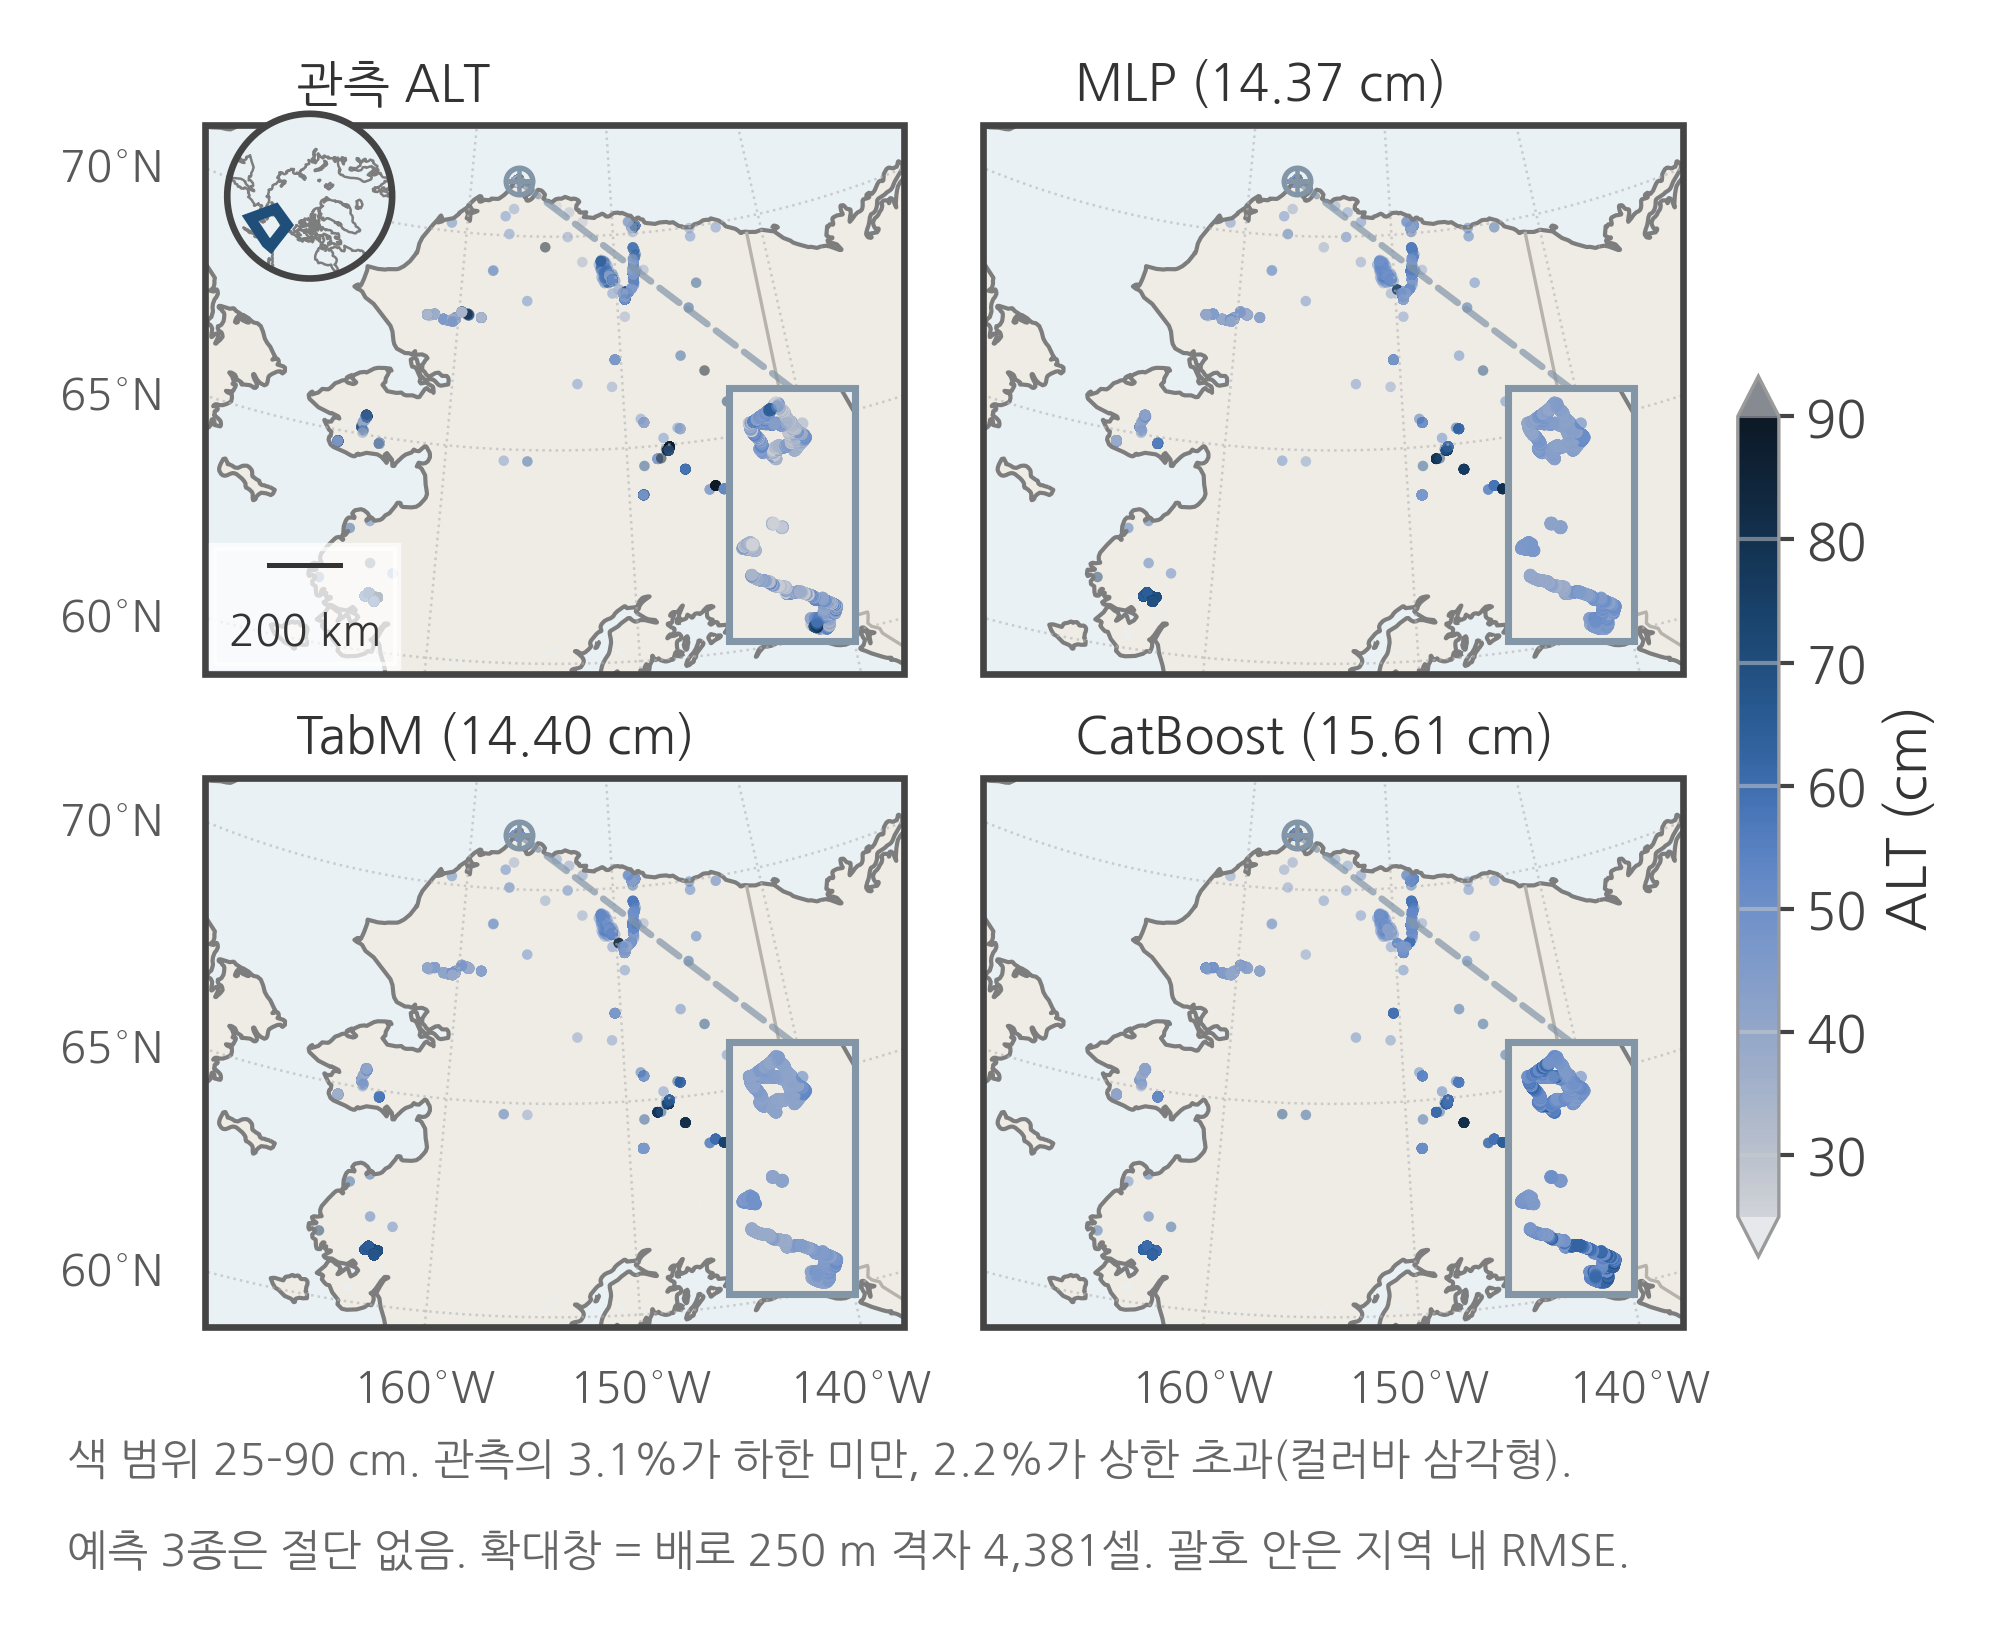
\includegraphics[width=\linewidth]{../../outputs/figures/s1_baseline/alaska_obs_vs_pred_maps.png}
  \caption{알래스카 ALT 예측 지도와 관측 밀집 inset. 예측장은 광역이나 관측 라벨은 소수 사이트에 집중된다.}
  \label{fig:s1maps}
\end{subfigure}\hfill
\begin{subfigure}[t]{0.485\textwidth}
  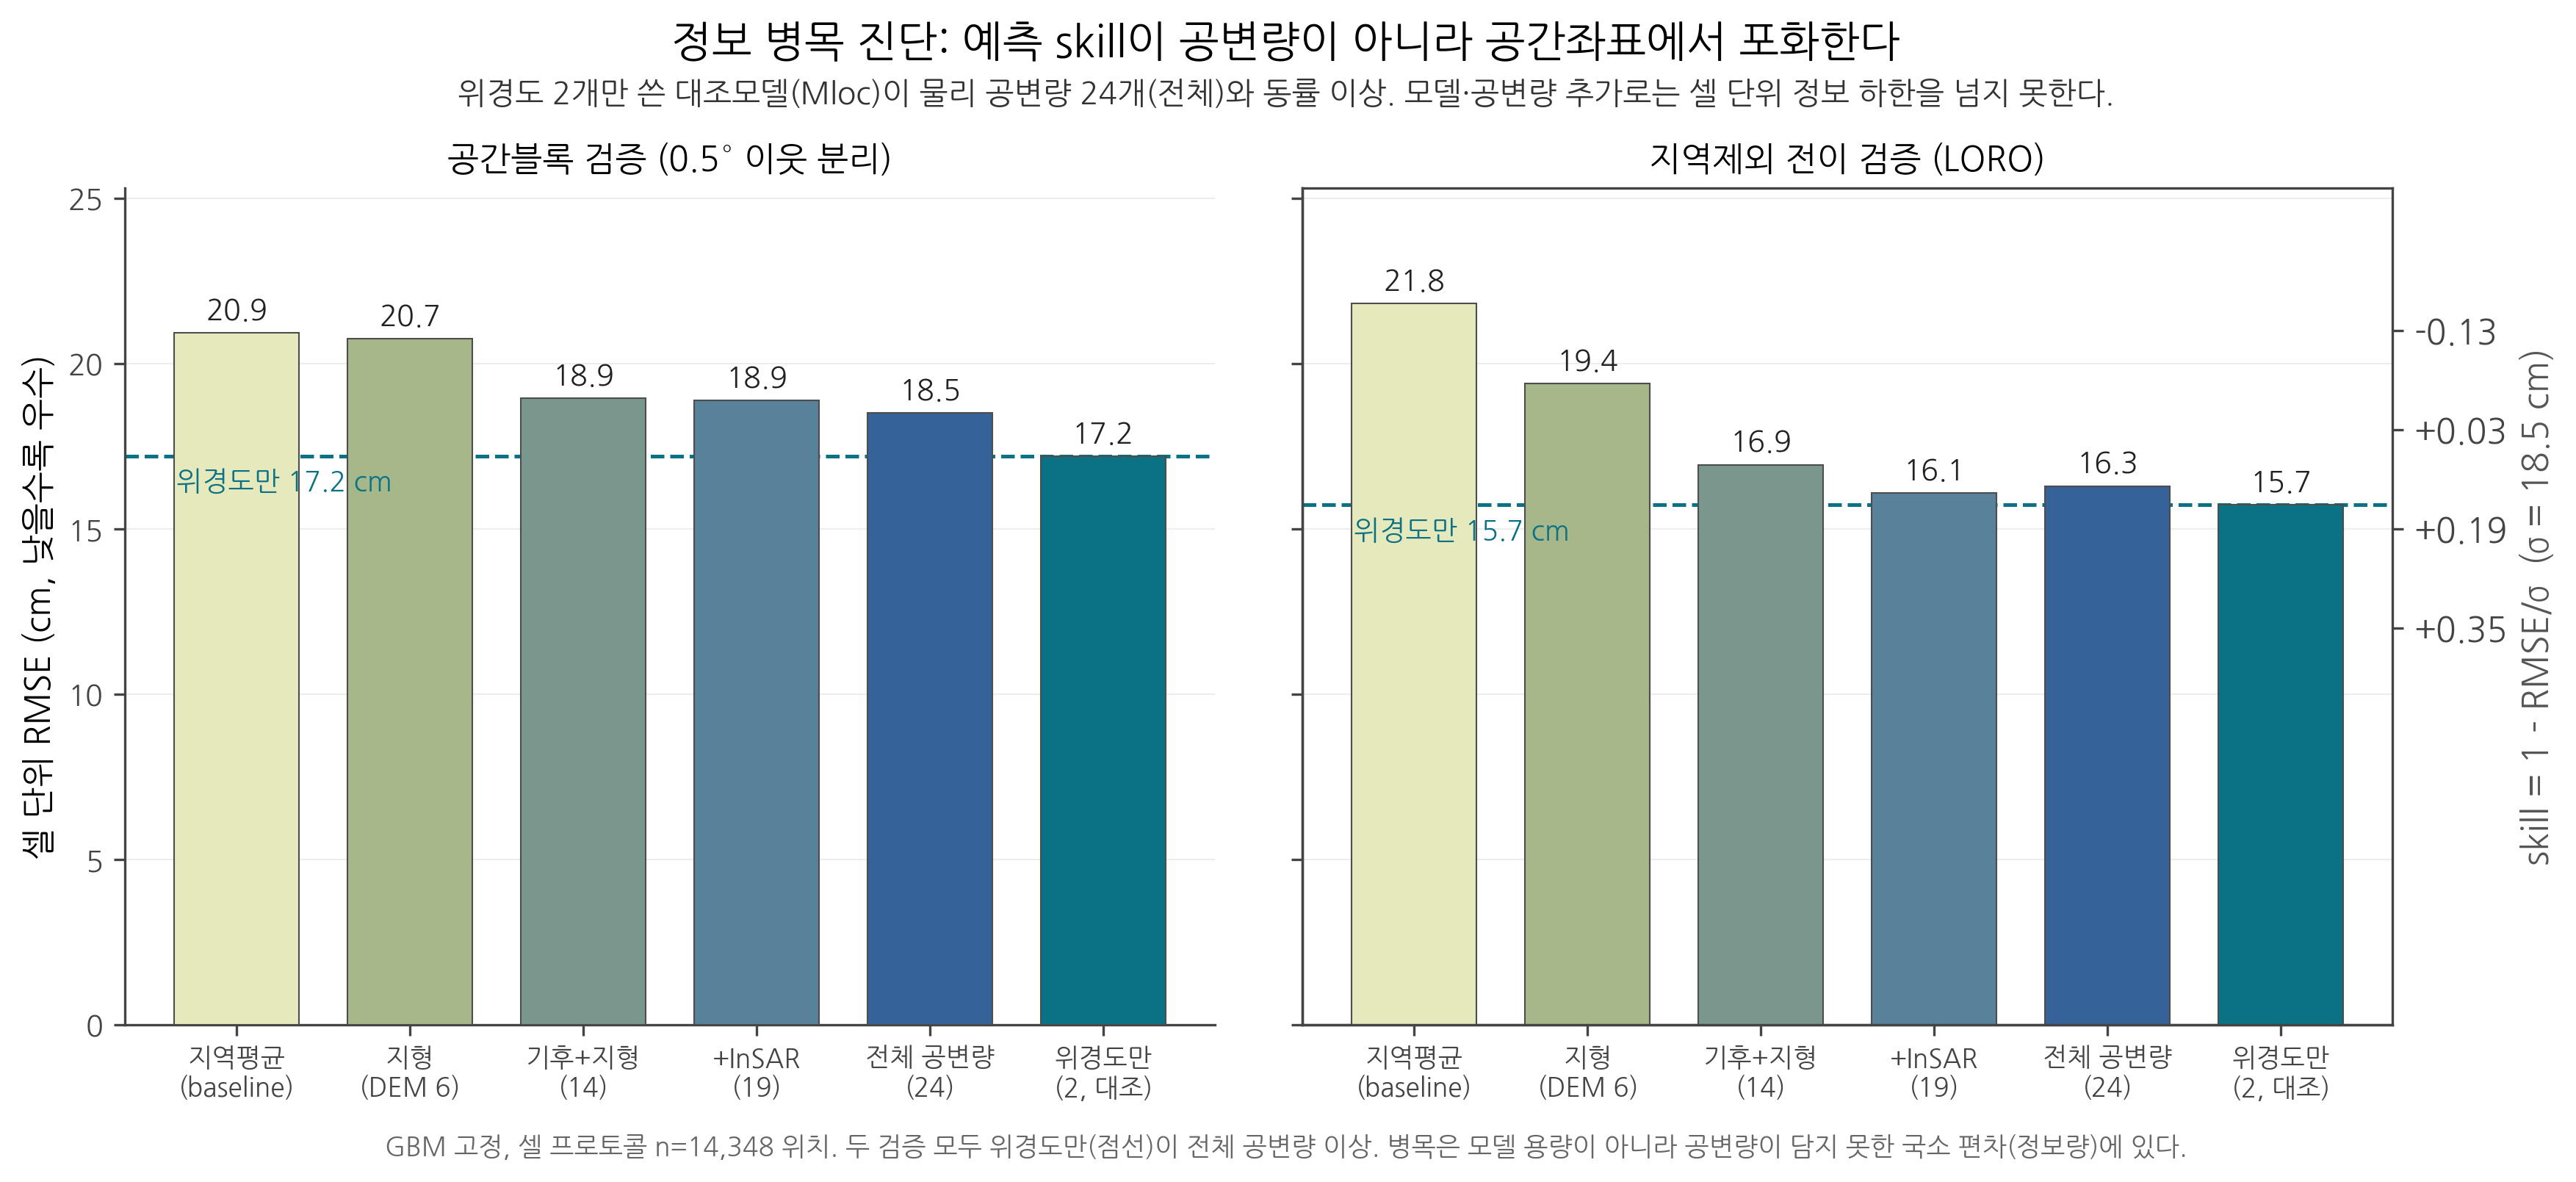
\includegraphics[width=\linewidth]{../../outputs/figures/06_deep_learning/alt_info_bottleneck.png}
  \caption{정보병목. 위경도 2피처 대조군이 물리·SAR 공변량 조합을 능가한다. 병목은 모델이 아니라 공변량 정보량이다.}
  \label{fig:bottleneck}
\end{subfigure}
\caption{in-domain 정확도와 정보병목 진단(\S4.1).}
\label{fig:accuracy}
\end{figure*}

\begin{figure*}[t]
\centering
\begin{subfigure}[t]{0.31\textwidth}
  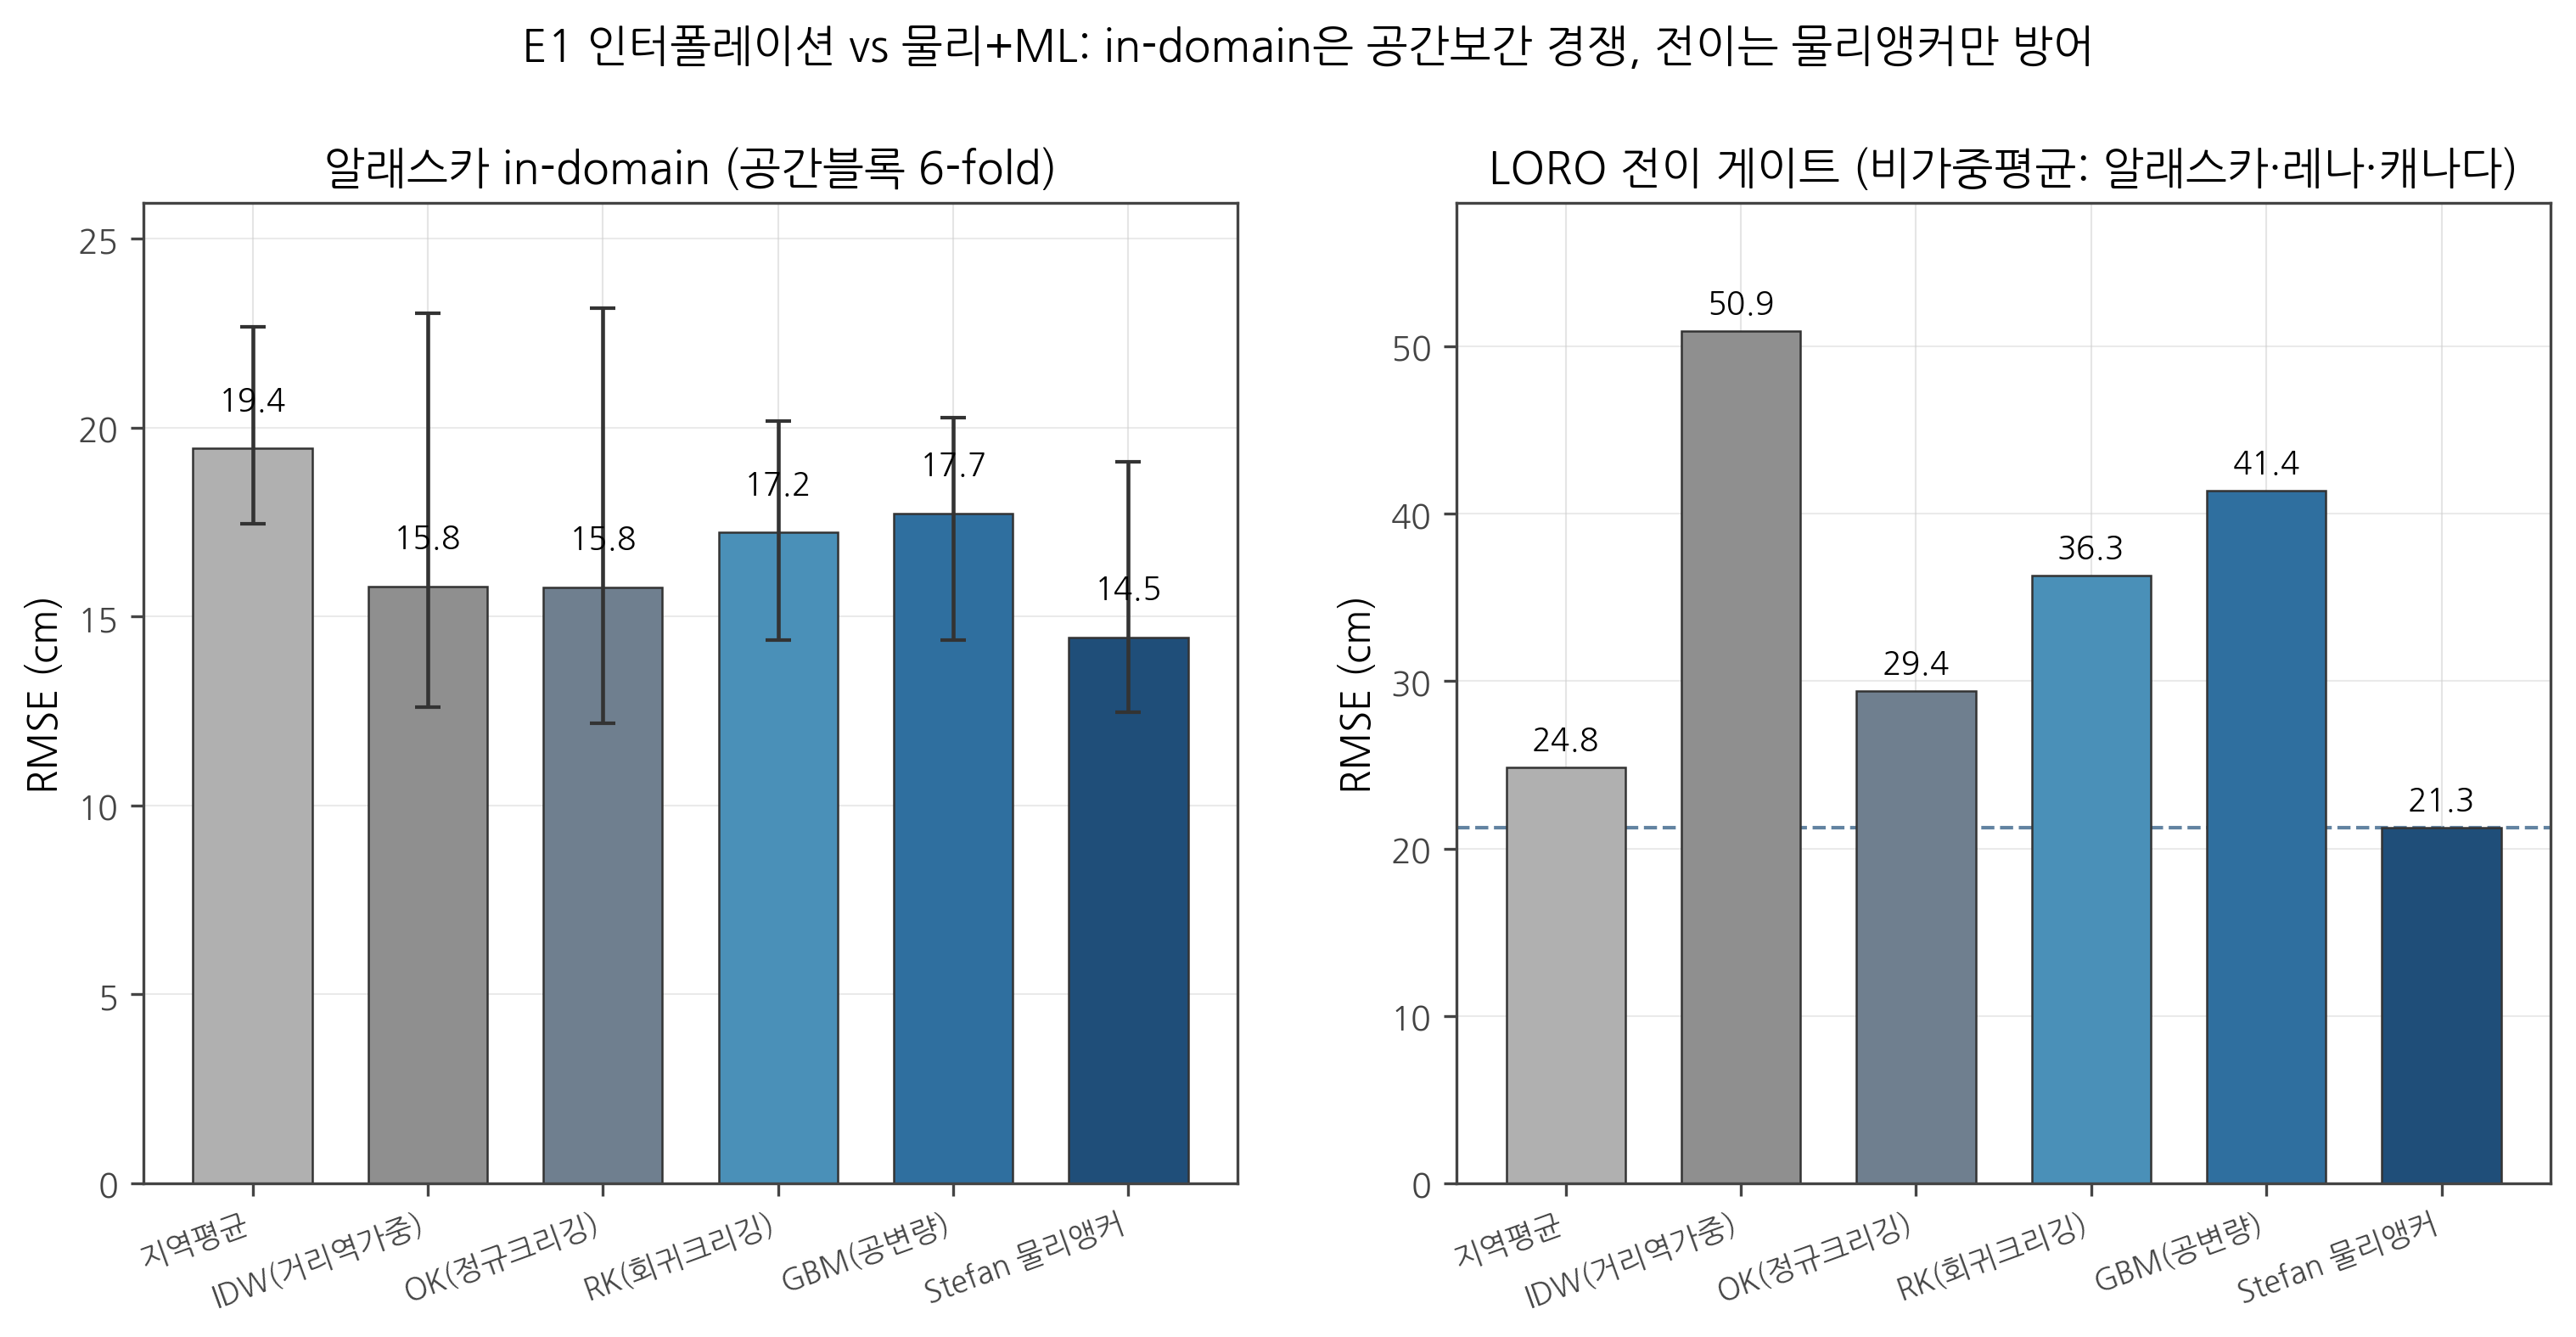
\includegraphics[width=\linewidth]{../../outputs/figures/e1_kriging/e1_rmse_bars.png}
  \caption{전이 붕괴 비교. 순수 ML·공간보간은 붕괴, 물리 앵커만 하한 유지(\S4.2).}
  \label{fig:kriging}
\end{subfigure}\hfill
\begin{subfigure}[t]{0.31\textwidth}
  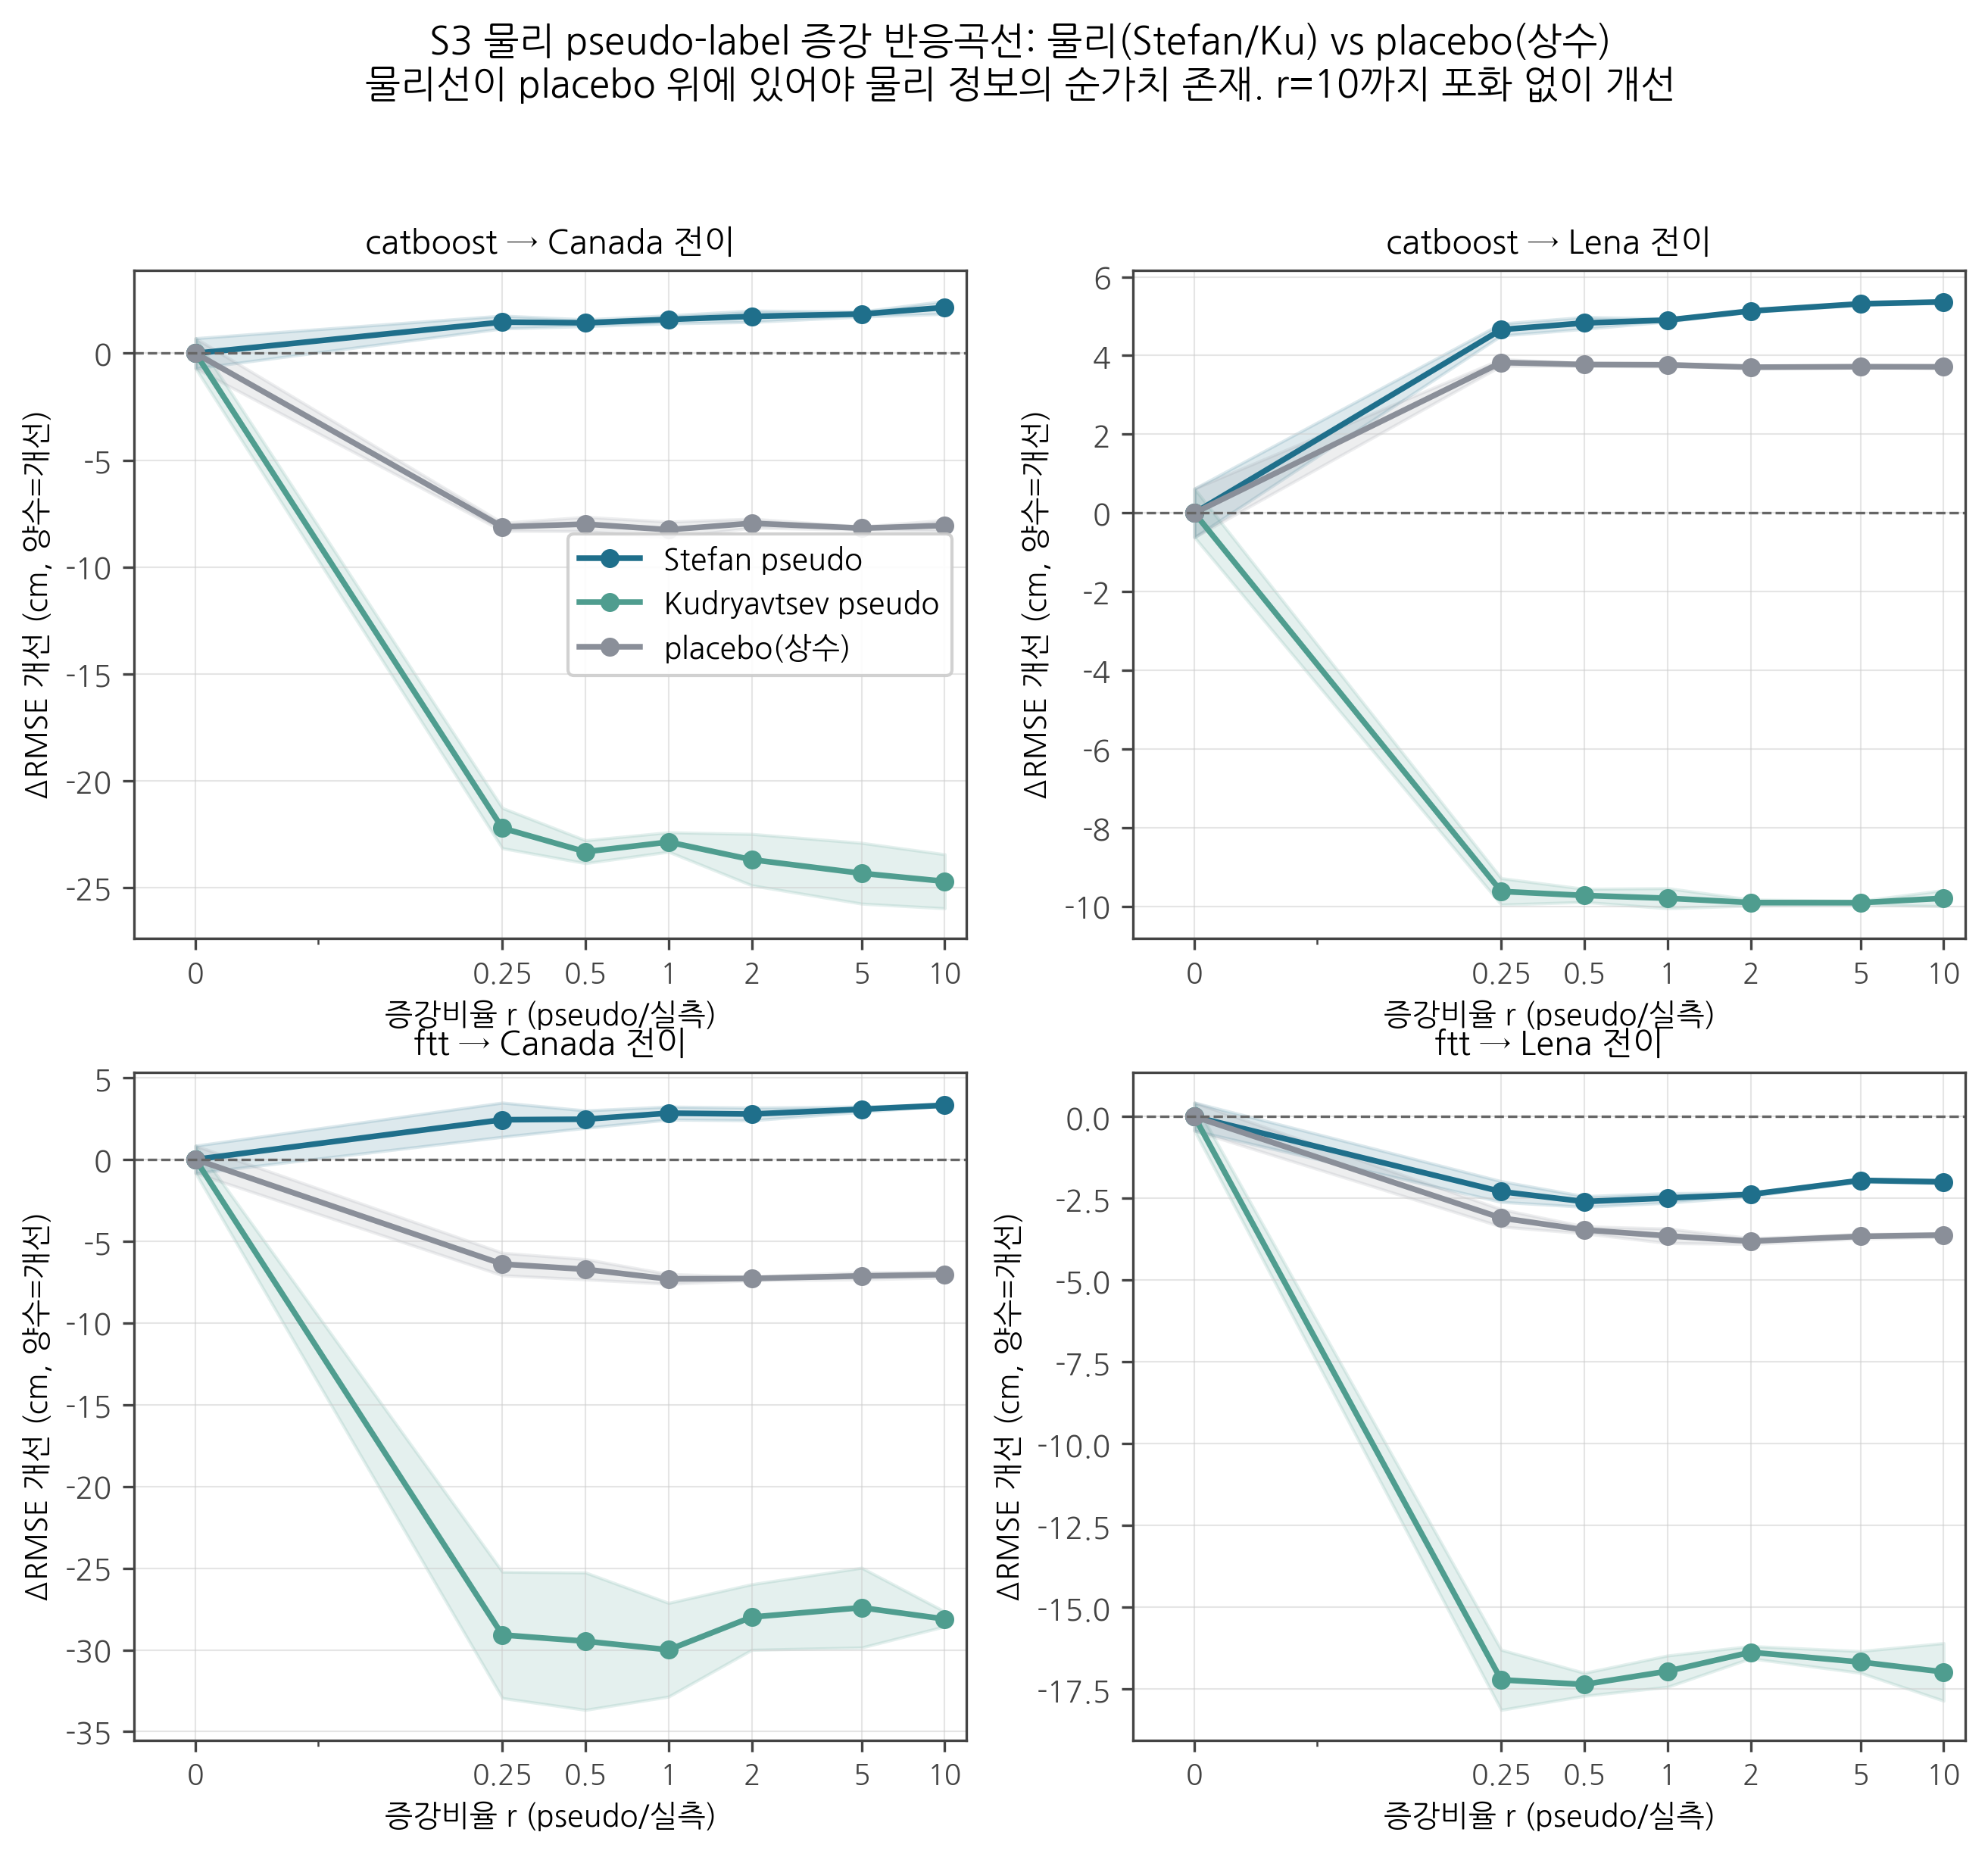
\includegraphics[width=\linewidth]{../../outputs/figures/s3_aug/aug_response_curves.png}
  \caption{증강 반응곡선. 부정확 물리는 $r$ 증가 시 악화된다(\S4.3).}
  \label{fig:aug}
\end{subfigure}\hfill
\begin{subfigure}[t]{0.34\textwidth}
  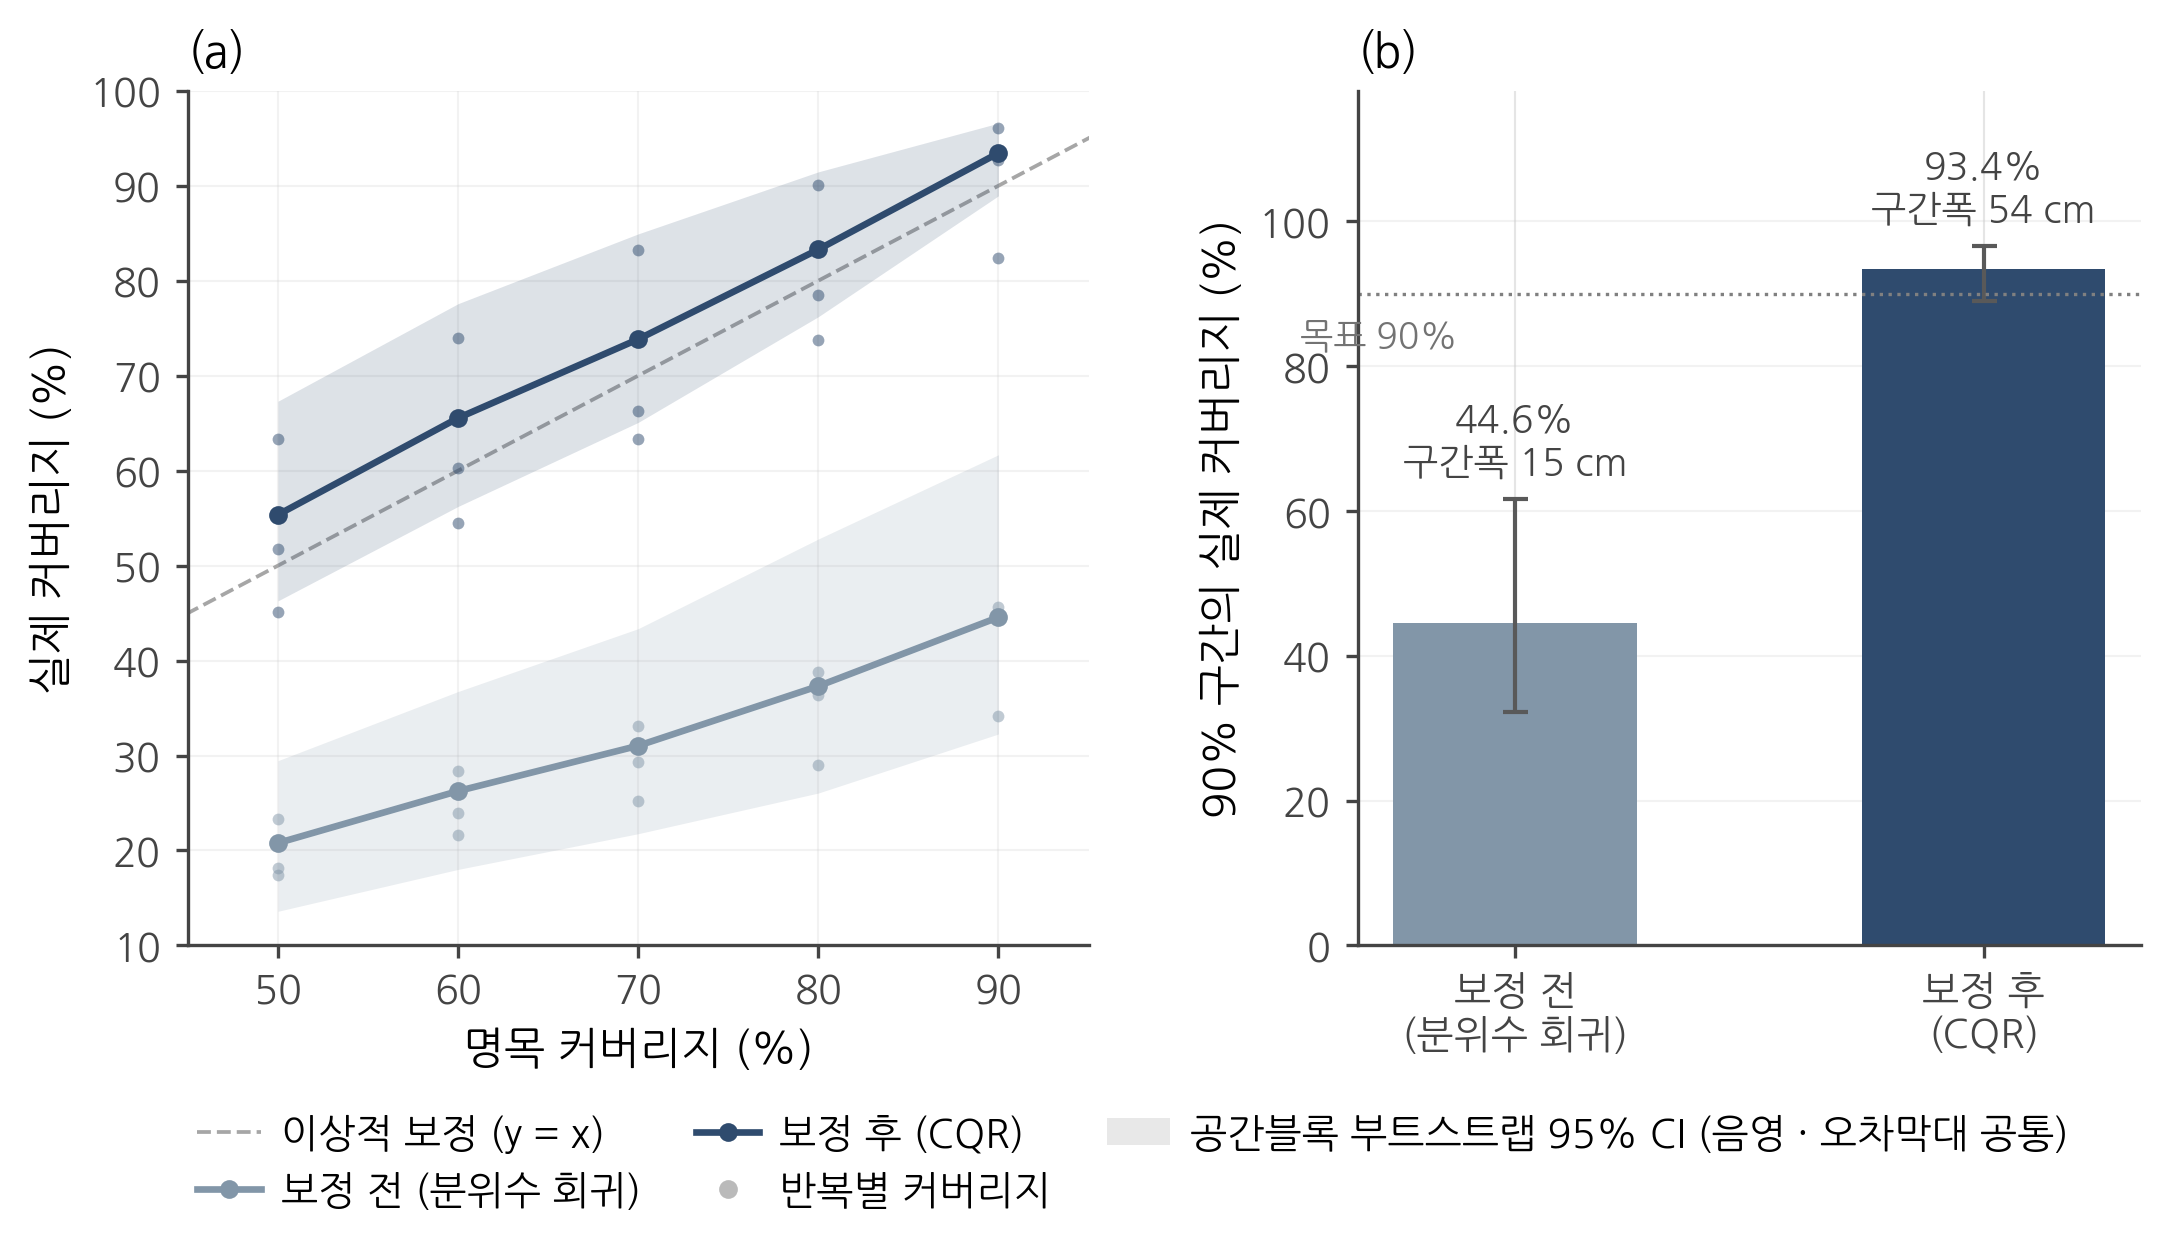
\includegraphics[width=\linewidth]{../../outputs/figures/s11_uq/s11_calibration_curve.png}
  \caption{보정 커버리지. raw 과신을 CQR이 목표 커버리지로 교정한다(\S4.4).}
  \label{fig:calib}
\end{subfigure}
\caption{전이·증강·보정 불확실성.}
\label{fig:transferrow}
\end{figure*}

% ===== 그림 묶음 2: 얕은3D·시계열·계절·KPDC =====
\begin{figure*}[t]
\centering
\begin{subfigure}[t]{0.30\textwidth}
  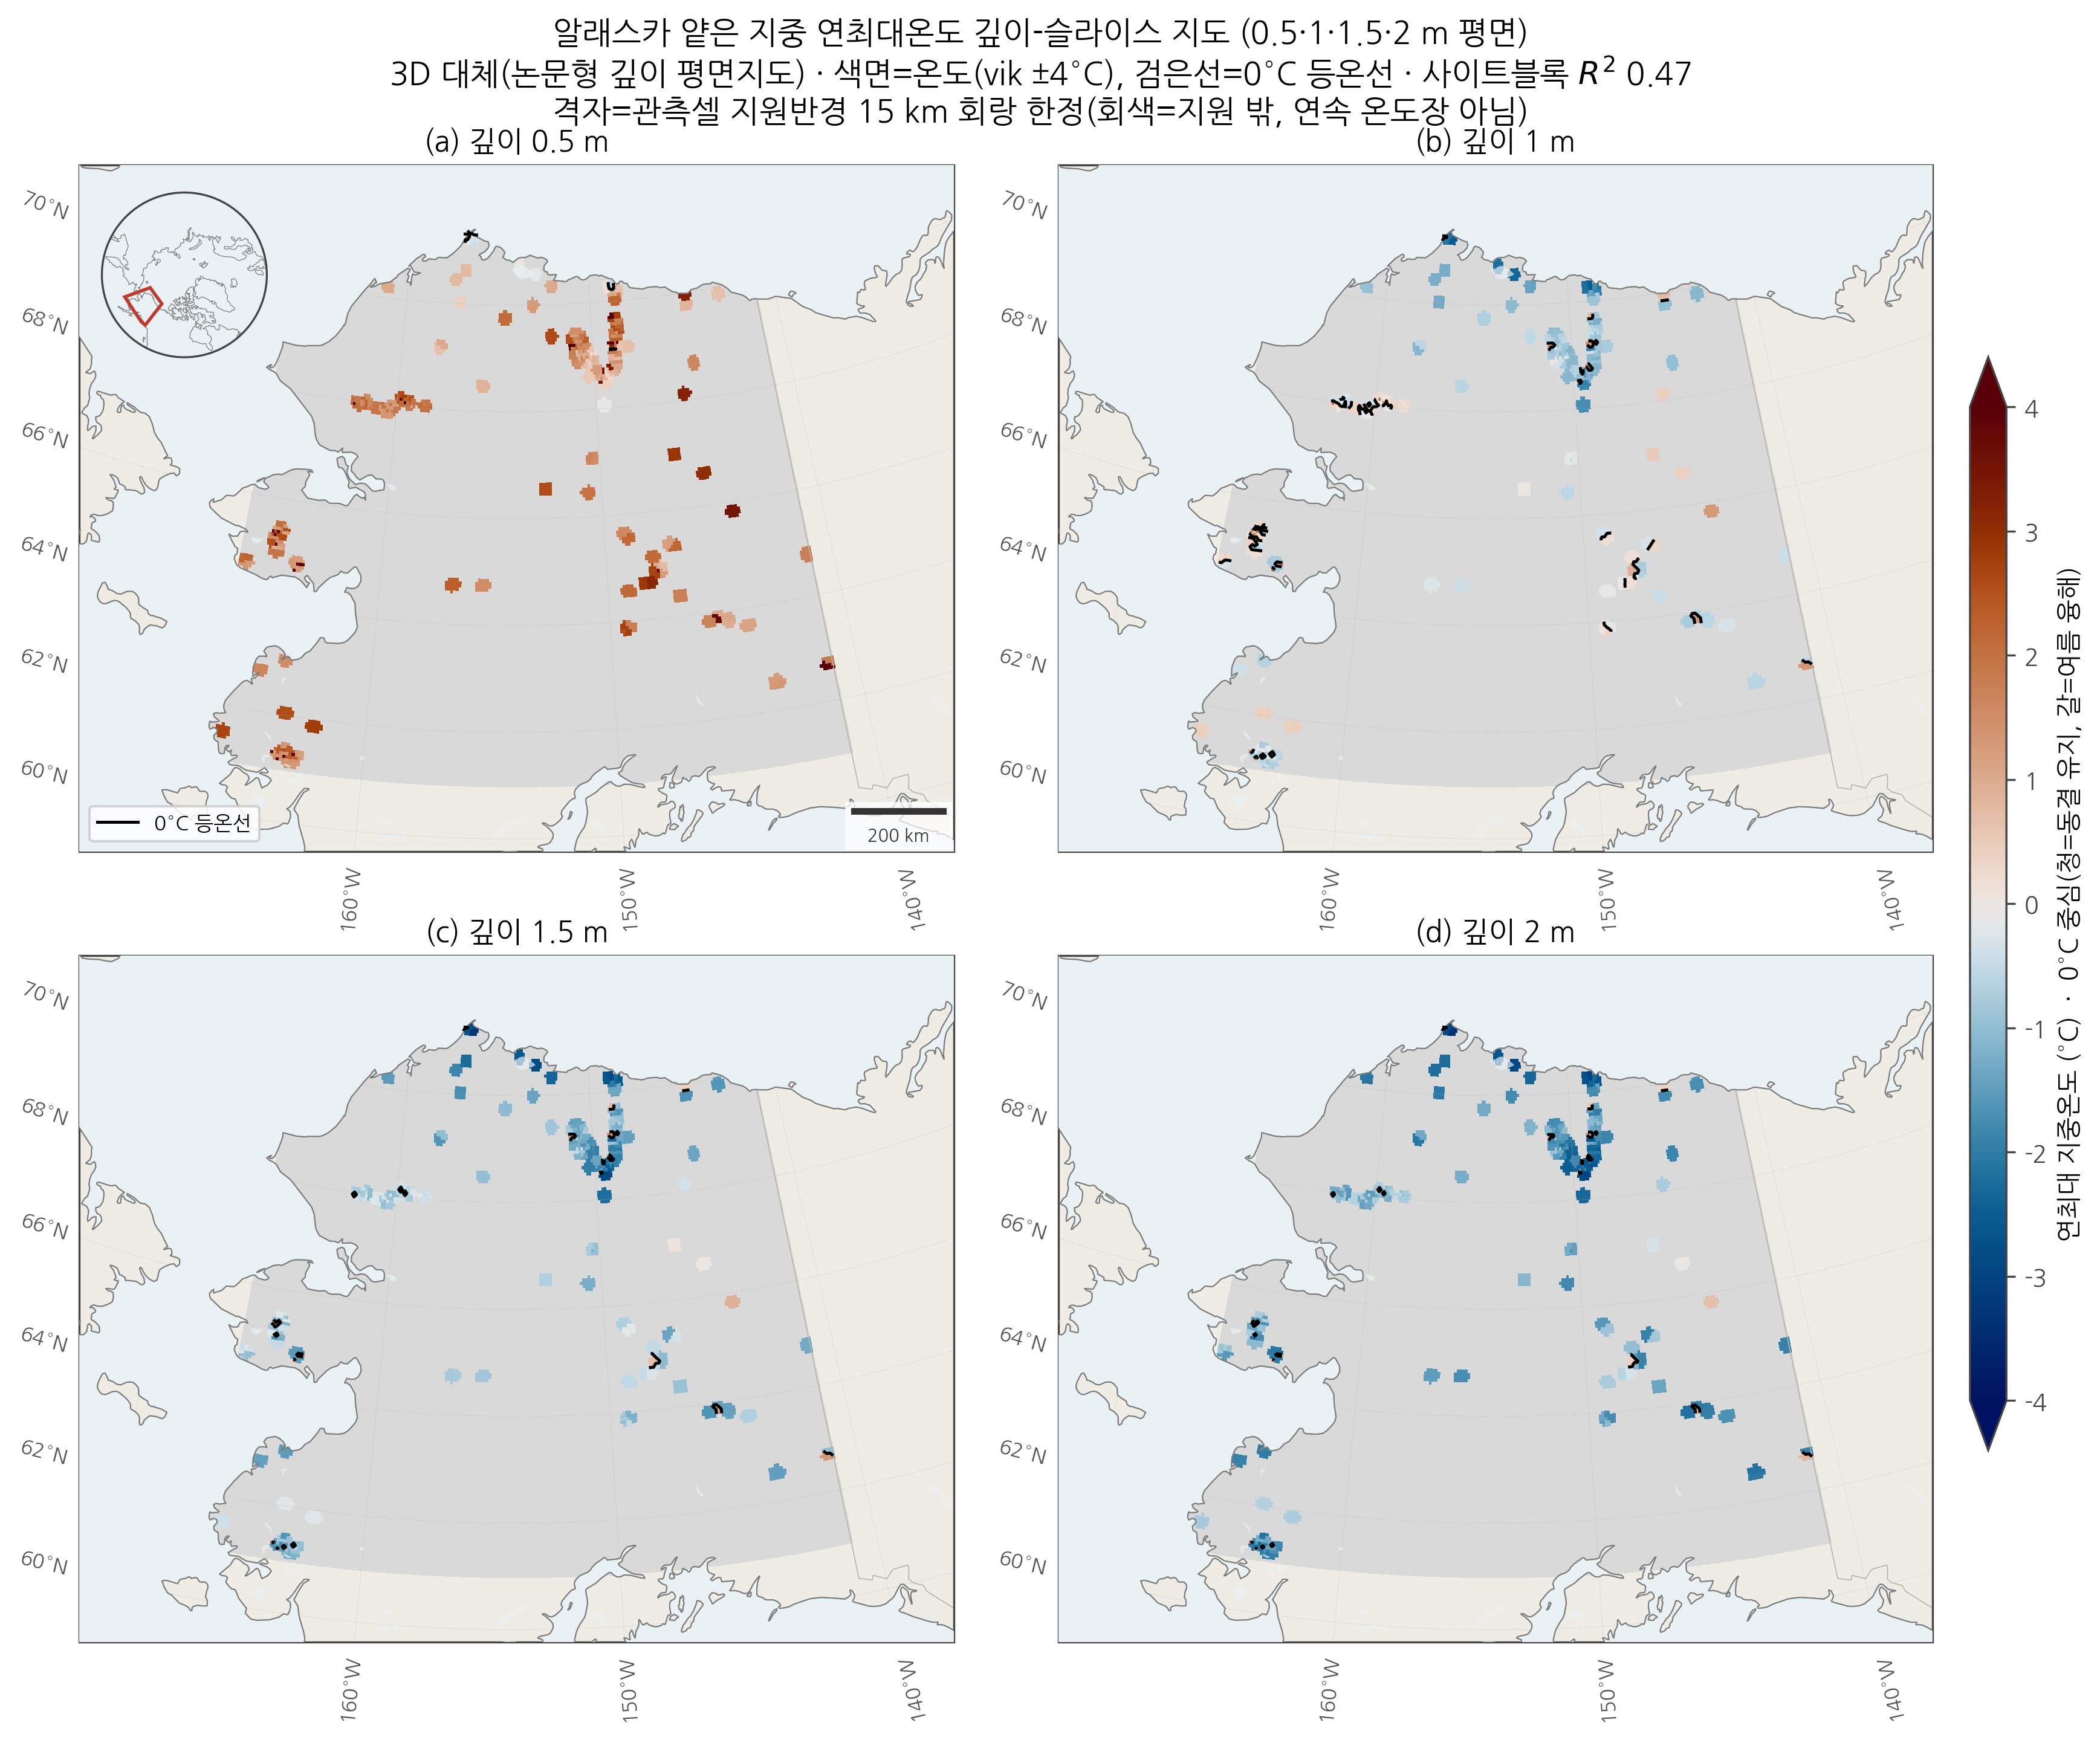
\includegraphics[width=\linewidth]{../../outputs/figures/s10_shallow3d/s10_depth_slices.png}
  \caption{얕은 3D 온도장 깊이 슬라이스($0\text{--}3\,\mathrm{m}$).}
  \label{fig:s10}
\end{subfigure}\hfill
\begin{subfigure}[t]{0.34\textwidth}
  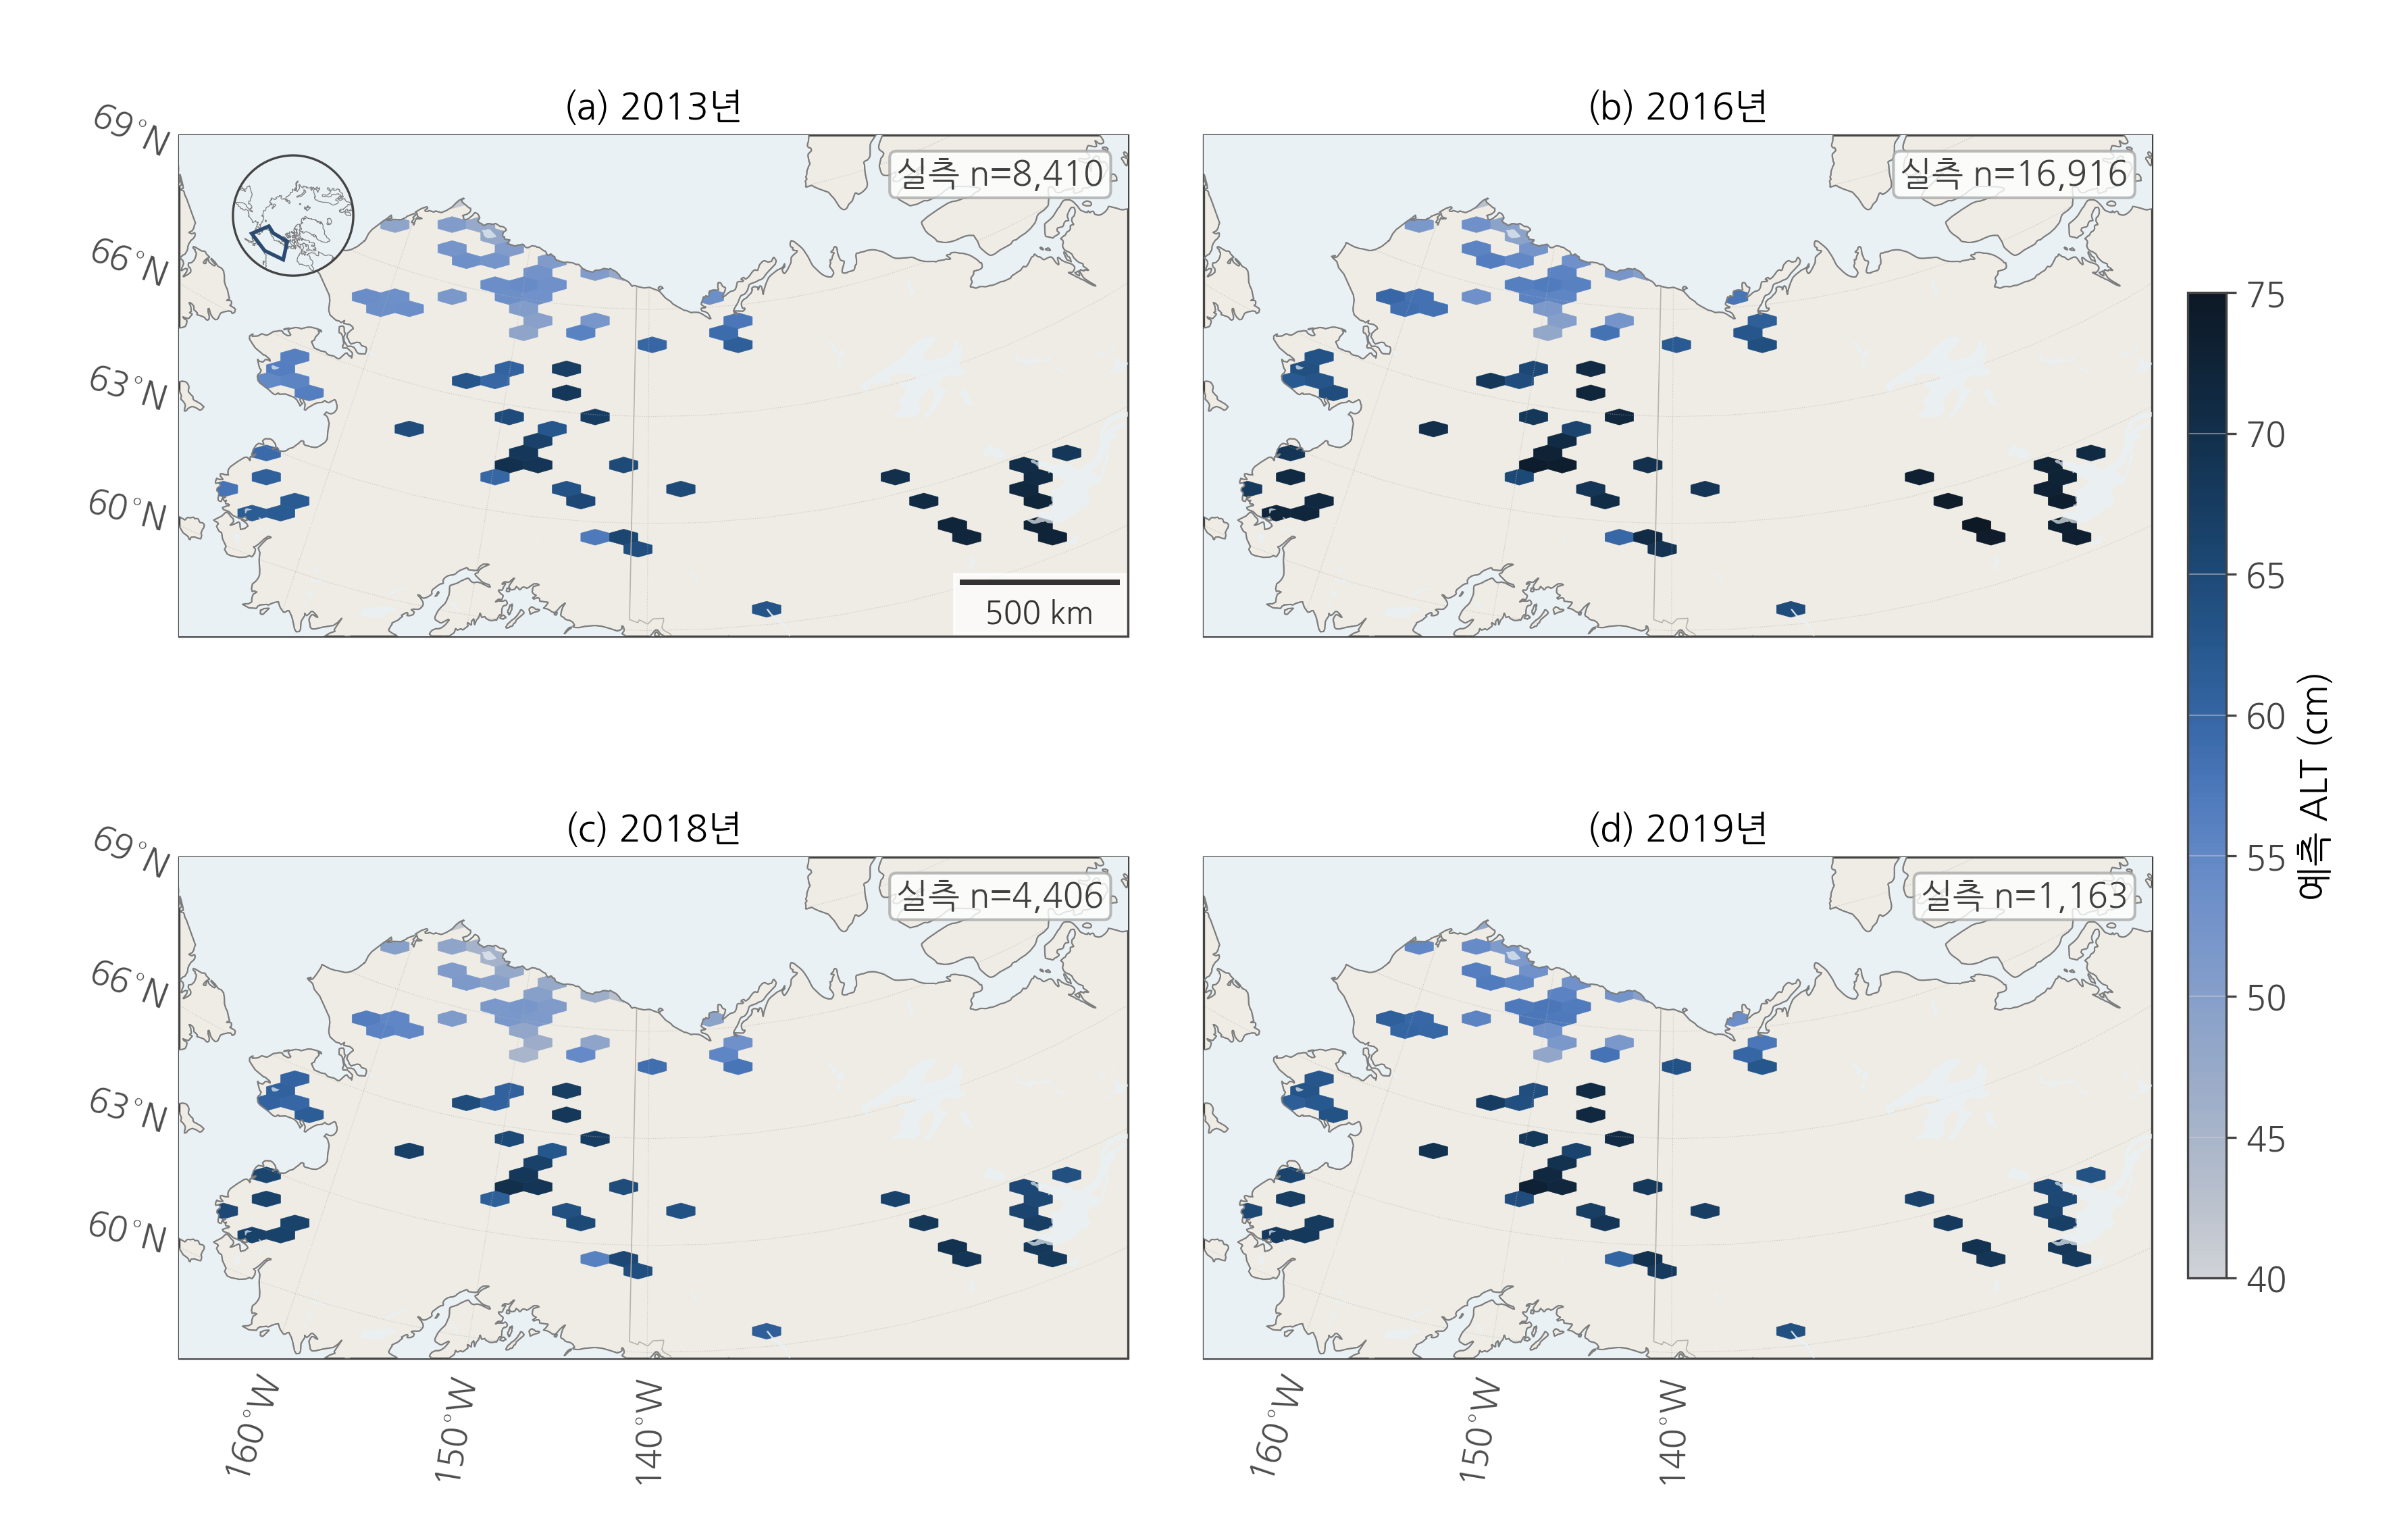
\includegraphics[width=\linewidth]{../../outputs/figures/s9_timelapse/alt_year_panels_v2.png}
  \caption{연별 ALT timelapse(2010--2024, forcing 시간 정합).}
  \label{fig:s9}
\end{subfigure}\hfill
\begin{subfigure}[t]{0.31\textwidth}
  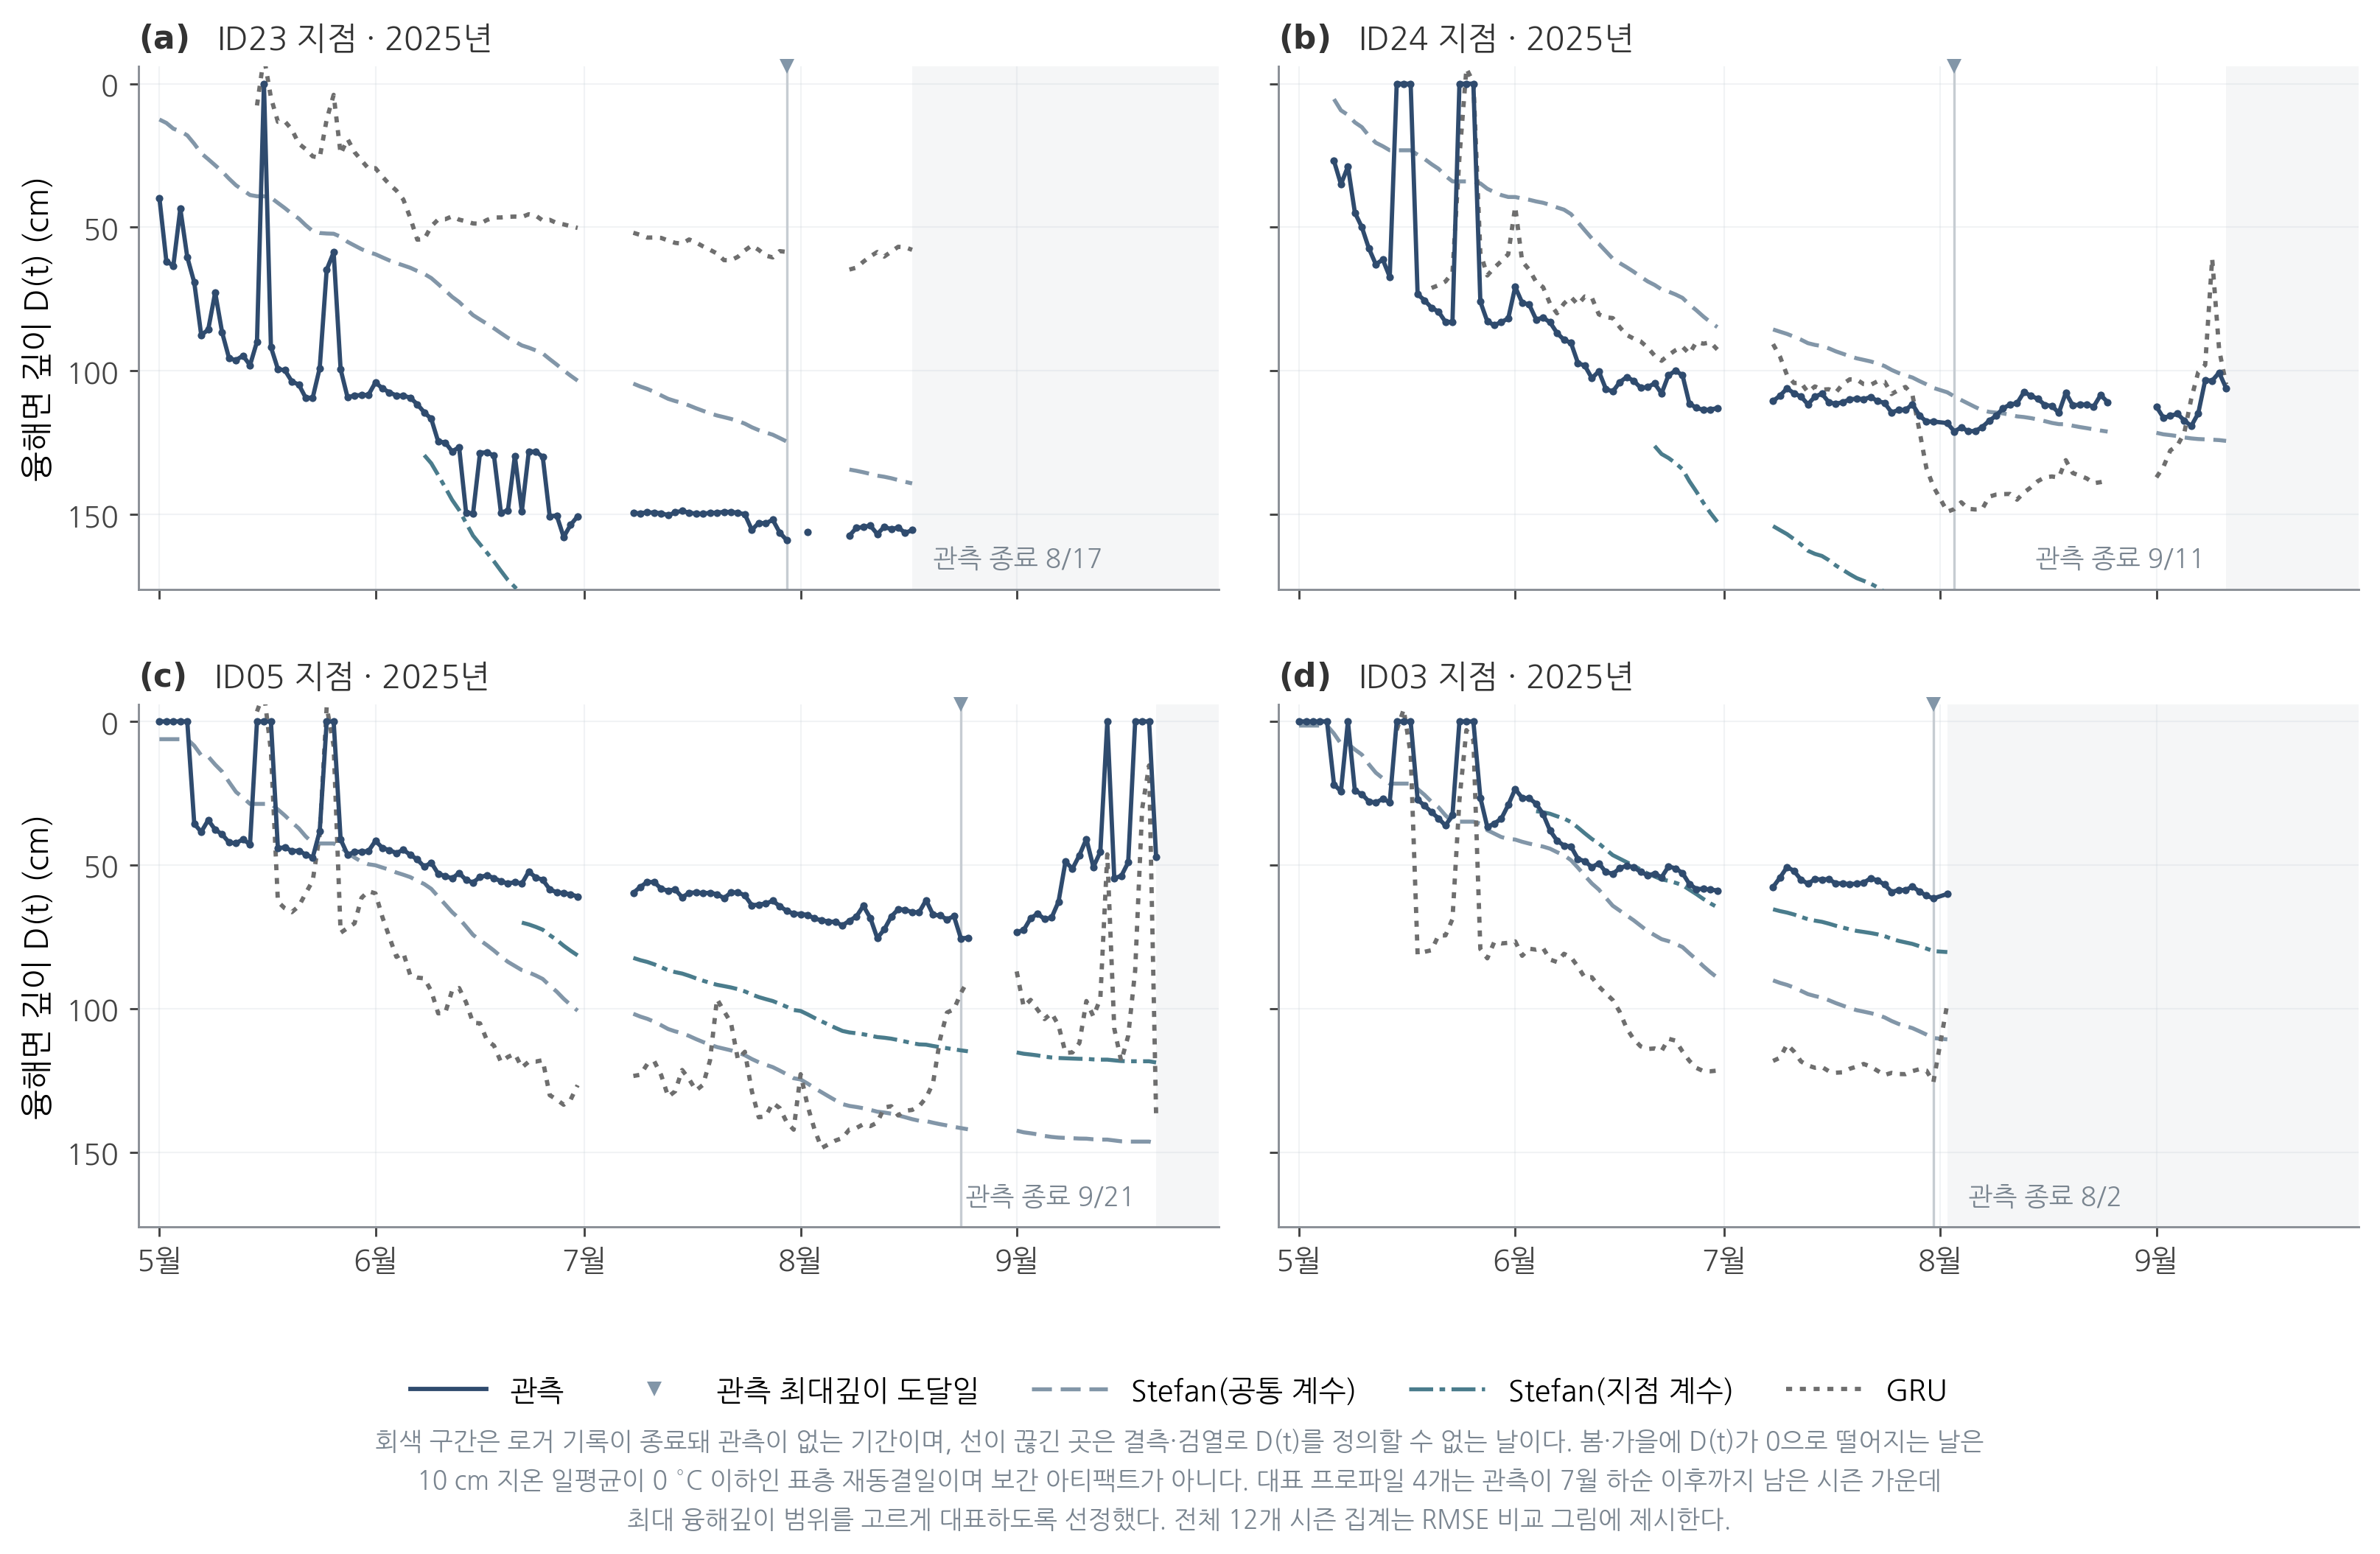
\includegraphics[width=\linewidth]{../../outputs/figures/e2_seasonal_dt/e2_dt_curves.png}
  \caption{계절내 $D(t)$ 곡선. 계절 구조는 예측 가능하다.}
  \label{fig:e2}
\end{subfigure}
\caption{얕은 3D 열구조와 시간 축 분석(\S4.5).}
\label{fig:timerow}
\end{figure*}

% ===== 그림 묶음 3: UQ 지도 · KPDC · PolSAR 국소데모 =====
\begin{figure*}[t]
\centering
\begin{subfigure}[t]{0.40\textwidth}
  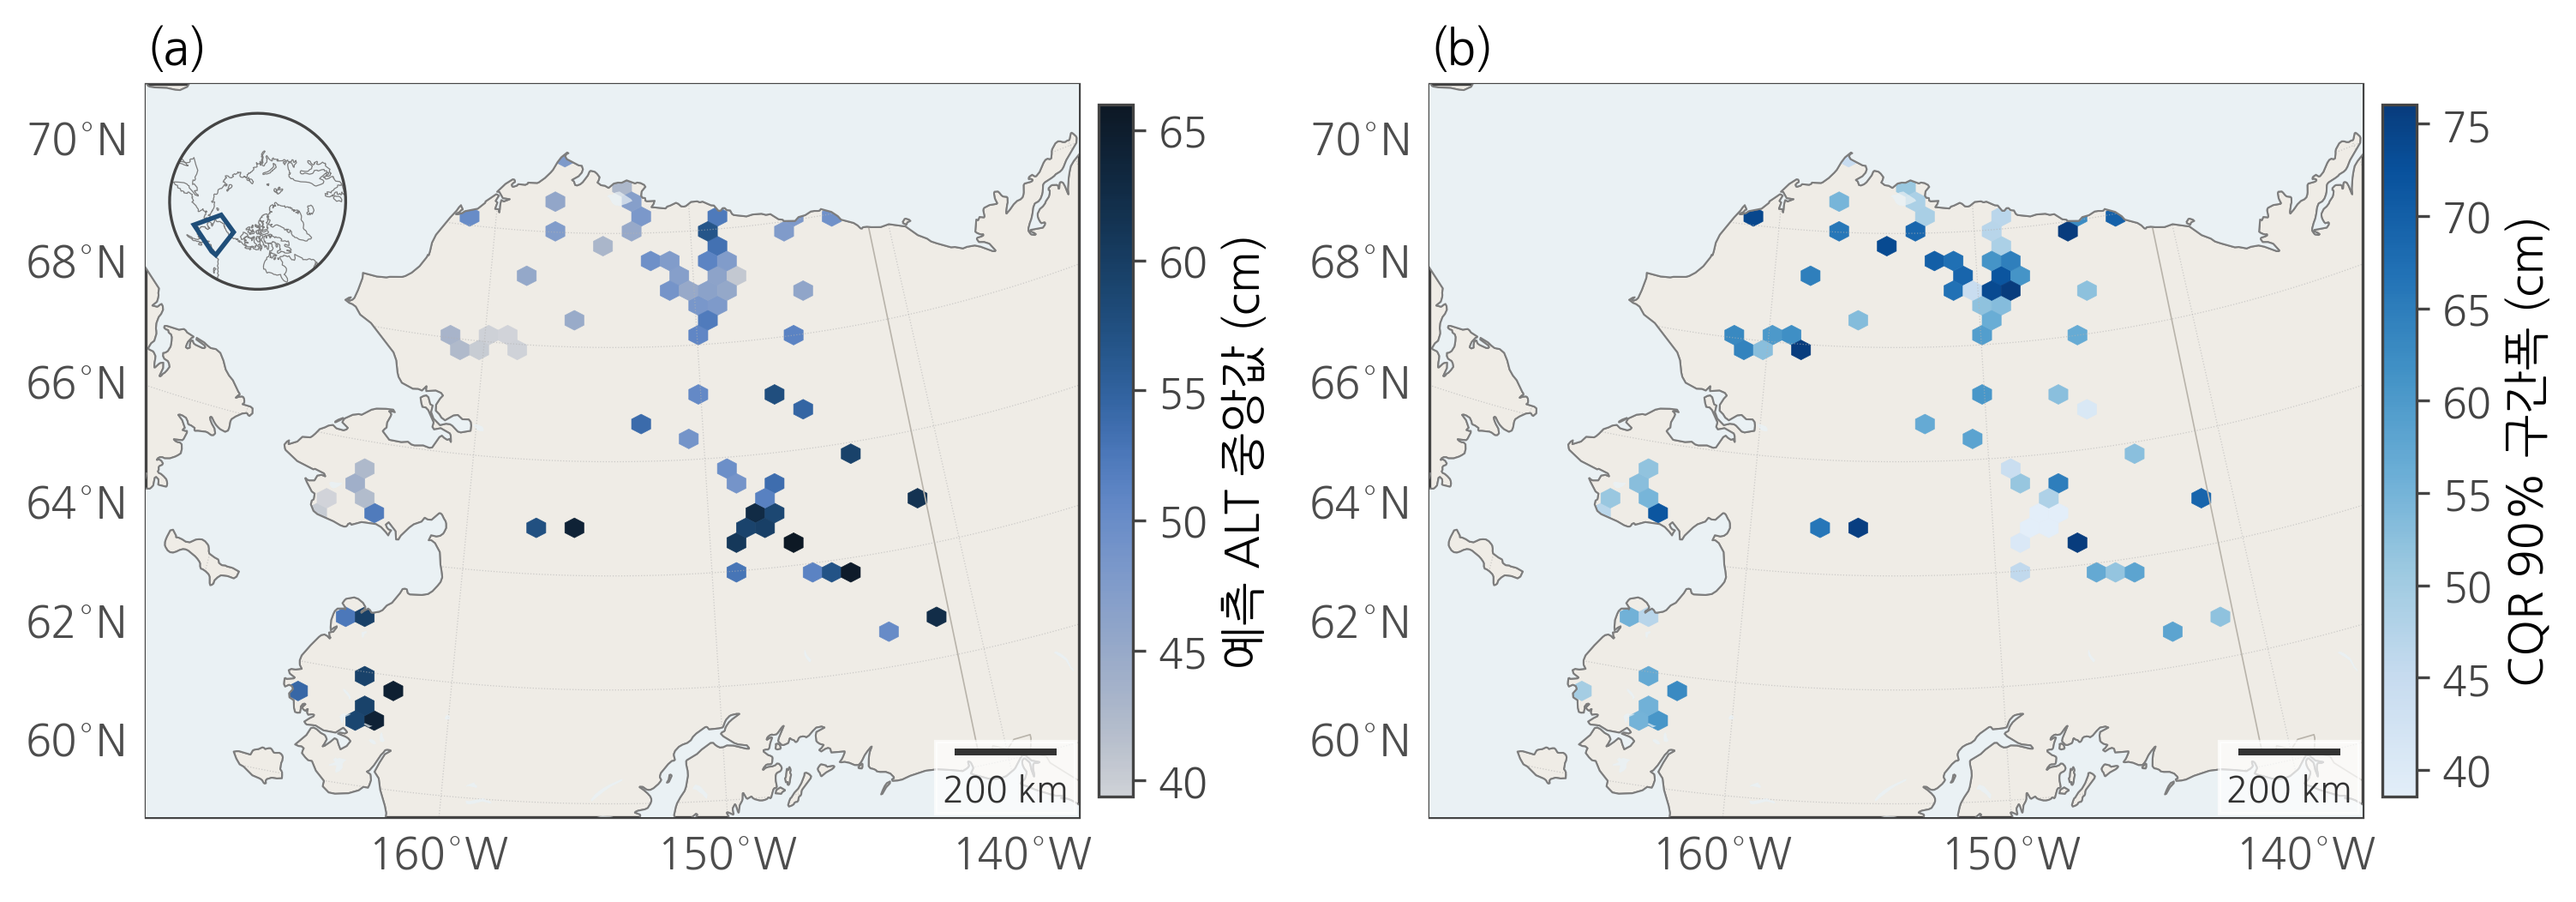
\includegraphics[width=\linewidth]{../../outputs/figures/s11_uq/s11_uq_maps.png}
  \caption{보정 예측구간 지도. AOA 비유사도가 큰 외삽 영역에서 구간이 넓어진다(\S4.4).}
  \label{fig:uqmaps}
\end{subfigure}\hfill
\begin{subfigure}[t]{0.27\textwidth}
  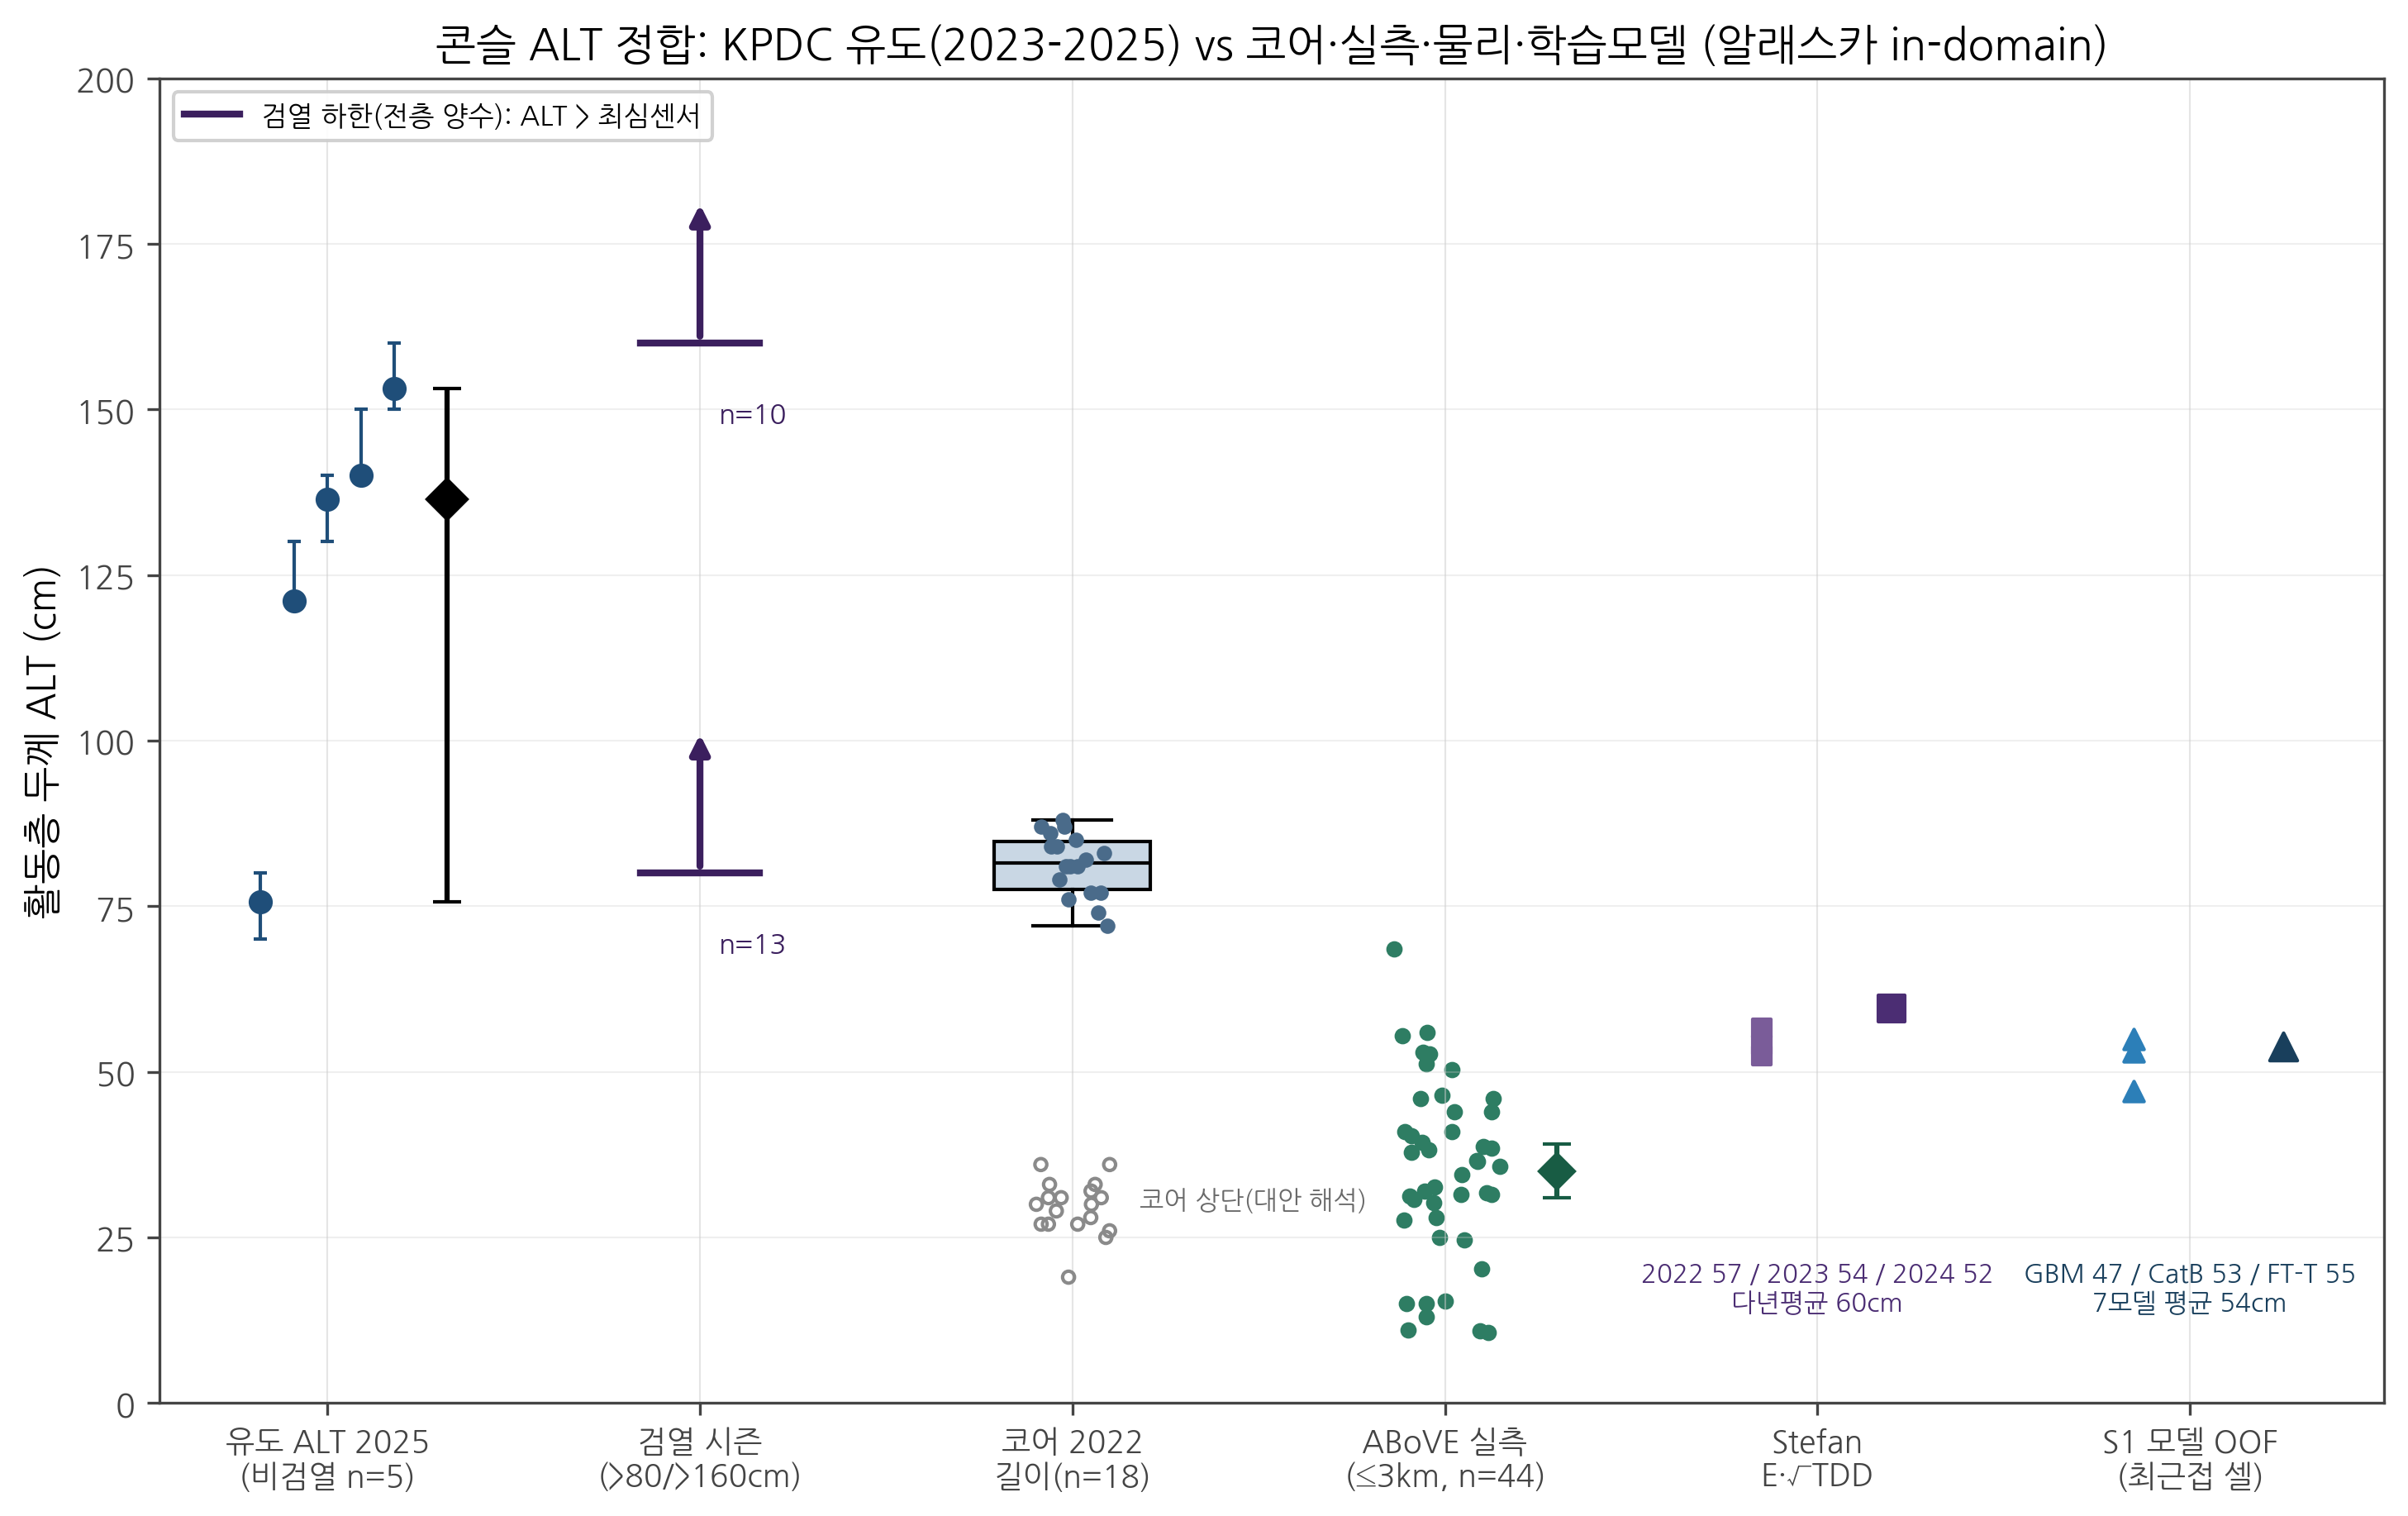
\includegraphics[width=\linewidth]{../../outputs/figures/s7_kpdc/s7_alt_comparison.png}
  \caption{KPDC 콘슬 ALT 유도 비교. 관측 방식에 따라 $35\text{--}153\,\mathrm{cm}$로 벌어진다(\S4.6).}
  \label{fig:kpdc}
\end{subfigure}\hfill
\begin{subfigure}[t]{0.30\textwidth}
  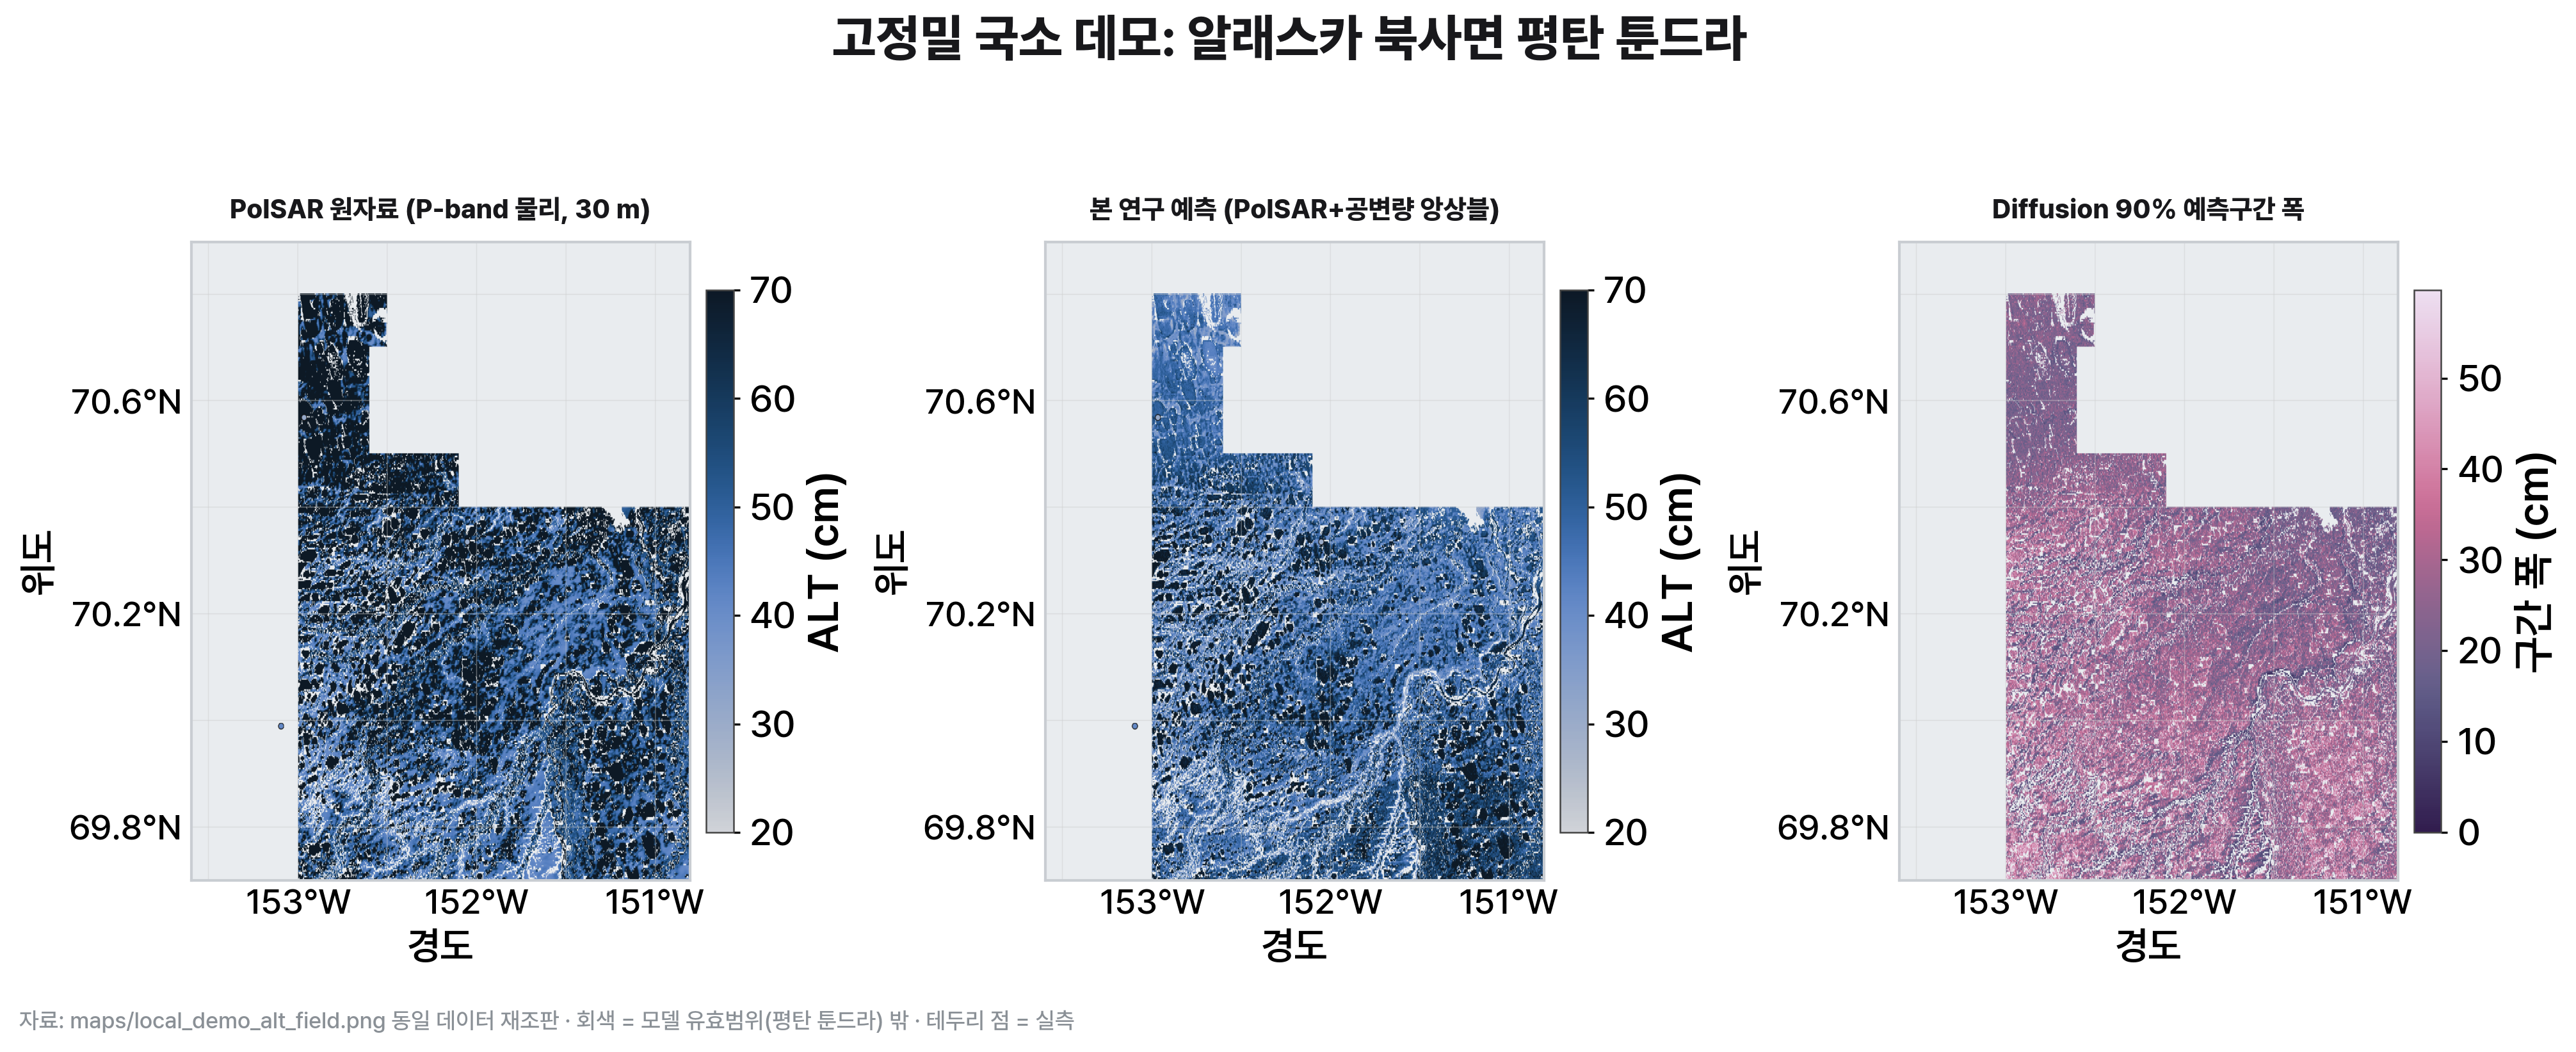
\includegraphics[width=\linewidth]{../../outputs/maps/local_demo_restyled.png}
  \caption{PolSAR $250\,\mathrm{m}$ 국소 데모. 고해상 물리관측의 공간 세부(\S2).}
  \label{fig:polsar}
\end{subfigure}
\caption{신뢰가능성·현장 검증·고해상 물리관측.}
\label{fig:uqrow}
\end{figure*}

\begin{multicols}{2}

% =====================================================================
\section{논의}
% =====================================================================

\subsection{강점}
본 프레임워크의 강점은 다섯 가지이다. 첫째, 관측기반 GeoAI로 순방향 시뮬레이션과 달리 관측 라벨로 직접 채점된다. 둘째, 물리 앵커가 전이의 하한을 담당해 순수 데이터 방법이 붕괴하는 지역 간 이동에서 유일하게 성능을 지킨다. 셋째, 보정 불확실성을 탑재해 예측구간이 통계적으로 유효하다. 넷째, 정통 지구통계(크리깅)를 정식 baseline으로 편입해 방법 비교가 공정하다. 다섯째, 얕은 3D·시계열·계절 $D(t)$·KPDC의 다각 검증으로 결과의 범위와 한계를 함께 규정한다.

\subsection{기존 연구 대비 차별성}
기존 연구가 순방향 시뮬레이션 위주였다면, 본 연구는 누설을 통제한 전이 벤치마크를 정면으로 다룬다. 물리·기계학습·지구통계를 동일 게이트에서 채점하고 전이 붕괴를 정량화한 것은 문헌에서 드물다. 관측기반 제품이 불확실성을 결여했다면, 본 연구는 conformal 보정으로 커버리지를 명시하고 그 in-domain 한계까지 보고한다. 물리정보 신경망 연구가 방법 신규성에 집중했다면, 본 연구는 구조 정교화가 전이를 개선하지 못한다는 부정 결과까지 담백히 보고해 어떤 정교화가 실효인지를 가려낸다.

구체적으로, GIPL2/SNAP 계열이 열전도 순방향으로 지온을 산출하되 지역 간 라벨 검증을 체계화하지 않은 데 비해, 본 연구는 Stefan 앵커를 관측 라벨로 fold-safe 채점하고 그 전이 하한을 수치로 제시한다. ESA CCI·Obu 등(2019)·Ran 등(2022)의 광역 지도 제품이 다년평균 격자값을 주되 예측구간을 주지 않는 데 비해, 본 연구는 각 셀에 보정된 커버리지와 AOA 표기를 부여한다. InterPIGNN·PI-LSTM 계열이 물리 제약을 신경망에 주입하는 방법 자체를 기여로 삼는 데 비해, 본 연구는 그러한 정교화(source-aware·mixture·잔차·사전학습)를 동일 게이트에서 시험하고, 전이에서 단일 물리 앵커를 넘지 못함을 진단으로 보고한다. 차별성의 핵심은 방법 하나의 우수성 주장이 아니라, 통제된 비교에서 무엇이 실효이고 무엇이 아닌지를 가려낸 데 있다.

\subsection{연구의 의의}
의의는 세 층위이다. 진단 층위에서, 정보병목이 모델이 아니라 공변량임을 밝혀 데이터 수집 우선순위(면적검증·target 라벨·조밀 지중온도)를 근거 있게 제시한다. 배포 층위에서, 물리 앵커$+$AOA 표기는 미검증 지역에도 하한을 보장하며 그대로 배포 가능한 하이브리드이다. 신뢰 층위에서, 보정 예측구간과 대표성 하한 명시는 사용자가 지도를 어디까지 믿을지 판단할 근거를 준다.

\subsection{한계와 극복 방안}
한계는 명확하며 각각의 극복 경로가 있다. 점검증 대표성 한계는 약 $10\text{--}12\,\mathrm{cm}$의 비가역 하한을 낳으므로, 다음 지렛대는 InSAR 면적평균 기준으로 검증 프로토콜 자체를 전환하고 셀당 다점 평균을 도입하는 것이다. 전이 병목은 모델 구조가 아니라 covariate shift이므로, 레나·캐나다에 target 라벨을 확보하는 것이 유일한 실효 지렛대이며 그 전까지는 물리 앵커$+$AOA 프레이밍을 유지한다. 계절 $D(t)$의 2년 소표본 한계는 forcing을 명시 입력으로 주고 조밀 지중온도를 확충하면 완화된다. 공변량 정보병목은 미세지형 재파생(TWI·다중스케일 TPI·곡률), 지형$\times$기후 교호항, 동적 토양수분·적설 절연항으로 완화를 시도한다.

\subsection{성능의 포지셔닝}
누설을 통제한 평가에서 본 프레임워크의 in-domain 성능은 물리기반 검증군(문헌 사이트 직접대조 RMSE $14\text{--}18\,\mathrm{cm}$ 대역)과 동일 대역이며 대표성 하한에 근접한다. 최소오차 주장은 하지 않는다. 차별점은 정확도 수치가 아니라 방법론에 있다. 전이 붕괴의 정량 규명(구조 정교화의 부정 결과 포함), 보정 불확실성, 얕은 3D, 계절내 $D(t)$의 예측가능성 구조 분리이다.

% =====================================================================
\section{결론}
% =====================================================================
관측이 소수 사이트에 초집중된 조건에서 영구동토 ALT를 광역 추정하려면, 정확도 경쟁만으로는 부족하고 정보병목·전이·신뢰가능성을 함께 규명해야 한다. 본 연구는 물리 앵커·기계학습·지구통계를 누설통제 아래 동일하게 채점해, 정확도 병목이 공변량 정보량이고 전이 병목이 covariate shift임을 정량적으로 보였다. 물리 앵커는 순수 데이터 방법이 붕괴하는 전이에서 유일하게 하한을 지키며, conformal 보정은 예측구간에 통계적 유효성을 부여한다. 이 진단은 다음 단계 데이터 수집(면적검증·target 라벨·조밀 지중온도)의 우선순위를 근거 있게 지시한다. 본 프레임워크는 그 자체로 배포 가능한 하이브리드이자, 신뢰가능한 극지 ALT 지도를 향한 진단 도구이다.

% =====================================================================
\section*{참고문헌}
% =====================================================================
{\footnotesize
\begin{enumerate}[leftmargin=1.4em,itemsep=0.5pt,topsep=1pt,label={[\arabic*]}]
\item Nicolsky, D. et al. GIPL2 / SNAP permafrost thermal model. \textit{The Cryosphere}.
\item ESA CCI Permafrost. Active layer thickness and ground temperature products.
\item Obu, J. et al. (2019). Northern Hemisphere permafrost map. \textit{Earth-Sci. Rev.}
\item Ran, Y. et al. (2022). New high-resolution permafrost maps of the Northern Hemisphere. \textit{ESSD}.
\item InterPIGNN: physics-informed graph neural network for permafrost.
\item PI-LSTM: physics-informed LSTM for active layer / ground temperature.
\item Romanovsky, V., Osterkamp, T. Stefan solution for active layer thaw depth.
\item Meyer, H., Pebesma, E. (2021). Area of applicability of spatial prediction models. \textit{Methods Ecol. Evol.}
\item Romano, Y., Patterson, E., Candès, E. (2019). Conformalized quantile regression. \textit{NeurIPS}.
\item CALM / GTN-P. Circumpolar Active Layer Monitoring and Global Terrestrial Network for Permafrost.
\end{enumerate}
}

\end{multicols}

\vspace{2pt}
{\footnotesize\color{softgray}\noindent 재현 정보. 통합 스키마·누설테스트, 실측-only 토너먼트, 물리 baseline, 증강 반응곡선, source-aware, mixture, 종합표·UQ, 공간보간, 계절 $D(t)$, KPDC 결과의 전 산출 CSV는 저장소 \texttt{data/processed/}에 있다. 대회 요건에 따라 KPDC 콘슬 자료를 주된 검증·해석 축으로 사용했다. 사전학습 모델·생성형 AI 사용 내역과 각 자료원의 라이선스·기간·해상도는 제출 시 별첨 표로 명시한다.}

\end{document}
